\documentclass[11pt]{article}
\usepackage[margin=1in]{geometry}
\usepackage{setspace}
\usepackage{fancyhdr}
\usepackage{graphicx}
\usepackage{float} % optional (for H placement)
\usepackage{hyperref}
\usepackage{longtable}
\usepackage{booktabs}
\usepackage{tabularx}
\usepackage{array}
\pagestyle{fancy}
\setlength{\headheight}{14pt}
\fancyhf{} % clear everything
\newcolumntype{Y}{>{\raggedright\arraybackslash}X}

% Header
\fancyhead[L]{One-Man-Business Multi-Agent Orchestrator System}
\fancyhead[R]{Group 8}

% Footer
\fancyfoot[C]{\thepage}
\begin{document}
\singlespacing
\begin{center}
{\LARGE \textbf{One-Man-Business Multi-Agent Orchestrator System}}\\[0.5em]

{\normalsize Rule-First, Prompt-Second Orchestration for Role-Aware Business Communication}\\
{\normalsize with Human Oversight, Risk Governance, and Responsible AI by Harness Design}

\vspace{1em}

Ewen Cheung Yi Wen$^{1}$, Chun Man Ng$^{1}$, Gabriella$^{1}$ and Jingyu Liao$^{1}$\\
{\small $^{1}$ School of Computing, National University of Singapore, Singapore}\\
{\small \{ewen.cheung, ng.chunman, gabriella, e0969003\}@u.nus.edu}
\end{center}

\vspace{1.5em}

\begin{center}
\textbf{Abstract}
\end{center}


\noindent
This report presents the One-Man-Business Multi-Agent Orchestrator, an AI system for managing trust-sensitive stakeholder communication on behalf of a solo entrepreneur. The paper is intentionally hybrid: it is both an application project for a real communication-management problem and a methodological study of bounded autonomy in agentic AI systems. Rather than relying on a single unconstrained assistant, the system decomposes each inbound message into role-aware retrieval, policy grounding, external research, memory access, reply drafting, and risk governance under a LangGraph supervisor. The design follows a rule-first, prompt-second philosophy: role-based access control (RBAC) is enforced through tool binding, approval gating is implemented in workflow structure, and LLM judgment is reserved for language generation and ambiguous semantic review. We interpret this control pattern as an approximate maximum expected utility (MEU) policy: the system automates low-risk replies when grounded evidence and policy clearance support autonomy, but escalates when the expected downside of commitments, disclosure, or liability exceeds the benefit of speed. On a 44-query policy benchmark, the policy agent achieves 90.9\% verdict accuracy and 100\% hard-constraint detection, with a 0.0\% hallucinated-supporting-rule rate under our overlap-based faithfulness proxy. In addition, selected verification suites yielded 104 passing tests covering risk checks, approval behavior, identity resolution, discount logic, and mocked end-to-end pipeline flows. The results support a focused but important claim: workflow-structured governance can make LLM-mediated business communication more grounded, reviewable, and deployment-aware, with the current study centering this claim on policy grounding, control-flow guarantees, and approval-governed autonomy.


\section{Introduction}
\subsection{Motivation and Problem Statement}
Solo entrepreneurs often face a difficult operational trade-off: they need to respond quickly across customers, suppliers, partners, and investors, but a single wrong message can create immediate financial or reputational harm. A customer discount promise can compress margin, an overconfident delivery assurance can create liability, and an investor-facing reply can expose information that should not be visible to other roles. These risks make the problem more demanding than generic ``chatbot reply generation'' because the system must reason over stakeholder type, internal business data, business policy, and escalation thresholds at the same time.

Single-agent LLM assistants are attractive because they are simple to deploy, but they offer limited structural control over access boundaries, intermediate reasoning, and approval routing. In practice, prompt-only constraints are brittle when the system must simultaneously retrieve private data, follow policy, and avoid risky commitments. This project therefore studies how an AI system can manage multi-stakeholder business communication for a solo entrepreneur while enforcing role-based data access, grounded policy compliance, risk governance, and human-in-the-loop approval for high-stakes decisions. In practical terms, the goal is not ``multi-agent for the sake of multi-agent''; it is bounded automation that can handle low-risk communication efficiently while keeping costly mistakes inside a reviewable control boundary across both website and Telegram entry channels.

\subsection{Contributions and Relevance to AI}
This work sits at the intersection of multi-agent systems, retrieval-augmented generation (RAG), LLM-based agents, structured output control, and responsible AI deployment\textsuperscript{[6,16,17,18,19]}. The report is intentionally positioned as both an AI application paper and a methodological paper: it addresses a concrete trust-sensitive business problem, but it also argues that workflow-structured control is a useful design pattern for bounded autonomy in agentic systems. Concretely, the paper makes five contributions:

\begin{itemize}
\item \textbf{Application contribution:} We formulate trust-sensitive, multi-stakeholder business communication for solo entrepreneurs as an AI systems problem that requires role awareness, policy grounding, escalation, and reviewable autonomy rather than generic answer generation alone.
\item \textbf{Application contribution:} We implement a deployable system that combines hybrid policy RAG, owner-authored SOUL/RULE context, three-layer memory, tool-scoped RBAC, and approval-gated response delivery across multiple channels.
\item \textbf{Methodological contribution:} We present a rule-first, prompt-second orchestration pattern in which safety-critical behavior is enforced by workflow structure and infrastructure-level controls rather than delegated entirely to prompting.
\item \textbf{Methodological contribution:} We argue that bounded replanning, escalation, and approval gating can be interpreted as an approximate MEU-style control policy for deciding when autonomy is acceptable and when human oversight should intervene.
\item \textbf{Evaluation contribution:} We combine a grounded policy benchmark with deterministic verification suites and mocked end-to-end pipeline tests to validate the parts of the system that are most central to controllability, policy grounding, and workflow-governed autonomy.
\end{itemize}

The broader AI relevance of the project is therefore twofold: practically, it addresses a real communication-management problem with deployment constraints; conceptually, it offers a case study of how planning, bounded autonomy, and responsible oversight can be operationalized in an agentic workflow.

\section{Literature Review / Related Work}

\subsection{Multi-Agent Systems and LLM Orchestration}
Multi-agent systems (MAS) have a long history in AI, focusing on communication, coordination, and cooperative problem-solving\textsuperscript{[1]}. Recent work on LLM-based agents has revived this line of research by treating language models as planners, tool users, and collaborators within larger control loops\textsuperscript{[2,16]}. Frameworks such as AutoGen\textsuperscript{[2]} and LangGraph\textsuperscript{[4]} make these agent workflows implementable in practice through graph-structured routing, state accumulation, and conditional fan-out/fan-in. Our design adopts a supervisor architecture in which a central orchestrator decomposes requests into specialized tasks and only routes to reply once required evidence has been collected. The design is also influenced by hierarchical task decomposition in classical planning, although our implementation is engineered around bounded replanning and typed state rather than formal task-planning guarantees\textsuperscript{[5]}.

\subsection{Retrieval-Augmented Generation (RAG)}
RAG improves LLM reliability by conditioning generation on retrieved evidence rather than on model parametric memory alone\textsuperscript{[6,17]}. Within RAG systems, hybrid retrieval and reranking are important because different failure modes arise at different stages: lexical gaps reduce recall, while poor rank ordering reduces precision. Prior work shows that cross-encoder reranking can improve document ranking quality over first-stage retrieval alone\textsuperscript{[8]}, and recent RAG evaluation work emphasizes that retrieval quality, answer grounding, and robustness must be measured separately\textsuperscript{[18,19]}. Our policy agent follows this logic by combining semantic search, lexical search, candidate merging, and cross-encoder reranking before policy evaluation.

\subsection{Risk Governance, Guardrails, and Human Oversight}
Deploying LLMs in business-critical settings requires more than output filtering. Human-AI interaction research consistently argues for calibrated automation, clear escalation, and preserved human control in consequential decisions\textsuperscript{[20,23]}. Guardrail frameworks such as NeMo Guardrails\textsuperscript{[10]} and Guardrails AI\textsuperscript{[11]} provide useful validation primitives, but they often operate near the model boundary rather than at the full workflow level. Our system therefore treats risk governance as a pipeline stage, not a post-processing convenience: a deterministic first layer catches explicit violations such as PII leakage, price commitments, and escalation triggers, while a semantic LLM layer reviews borderline cases for implied commitments, contradictions, and tone anomalies. This follows a defense-in-depth philosophy\textsuperscript{[12]} and better matches deployment settings in which some decisions should be blocked structurally rather than merely discouraged in prompting.

\subsection{Role-Based Access Control in AI Systems}
RBAC is well established in traditional software systems\textsuperscript{[13]}, but its application to LLM-powered tools remains comparatively underdeveloped. This matters because prompt injection attacks can cause models to ignore or reinterpret prompt-level restrictions\textsuperscript{[21,22]}. In business communication systems that retrieve internal data, this makes prompt-only access control an insufficient security boundary. Our system instead enforces RBAC at the tool-binding layer: the retrieval agent is only given the functions permitted for the sender's role, so unauthorized data access is blocked even if the model is manipulated or hallucinates an incorrect action. This design directly addresses the gap between conversational instruction following and infrastructure-enforced privilege separation.

\subsection{Conversational Memory and Context Management}
Maintaining coherent long-term context in multi-turn conversations remains challenging for LLM systems. Approaches range from simple sliding window buffers to structured memory systems with retrieval\textsuperscript{[14]}. Our system employs a three-layer memory architecture: short-term (recent messages), durable (long-term facts and preferences), and sender-specific profiles, with periodic compaction to manage context window budgets. This design is influenced by memory-augmented language models and the MemGPT architecture\textsuperscript{[15]}.

\subsection{Comparison with Alternative Approaches}
Compared with single-agent assistants, rule-based automations, and end-to-end retrieval systems, our architecture moves safety-critical functions such as RBAC and approval gating out of prompts and into workflow structure. This increases complexity and latency, but it improves modularity, auditability, and human control for trust-sensitive business communication. A detailed comparison is provided in Appendix~\ref{app:comparison}, and the evaluation section discusses how a fuller matched baseline study could be conducted in future work.

\section{Methodology}

\subsection{System Architecture and Pipeline Flow}
The system follows a supervisor-based multi-agent architecture implemented in LangGraph as a directed graph with bounded replanning. Each message passes through intake, orchestration, sub-agent execution, reply generation, approval checking, and risk evaluation before either automatic dispatch or hold-for-approval. The pipeline operates over a shared state object that accumulates sender role, memory context, task progress, reply metadata, and approval status across nodes. This design makes the control flow inspectable: instead of hiding retrieval, policy checks, and escalation logic inside one prompt, the workflow exposes where evidence is gathered, where rules are applied, and where human review can intervene. Figure~\ref{fig:system-architecture} shows the high-level flow, while Appendix~\ref{app:control-table} provides a compact stage-by-stage responsibility table.

\begin{figure}[H]
    \centering
    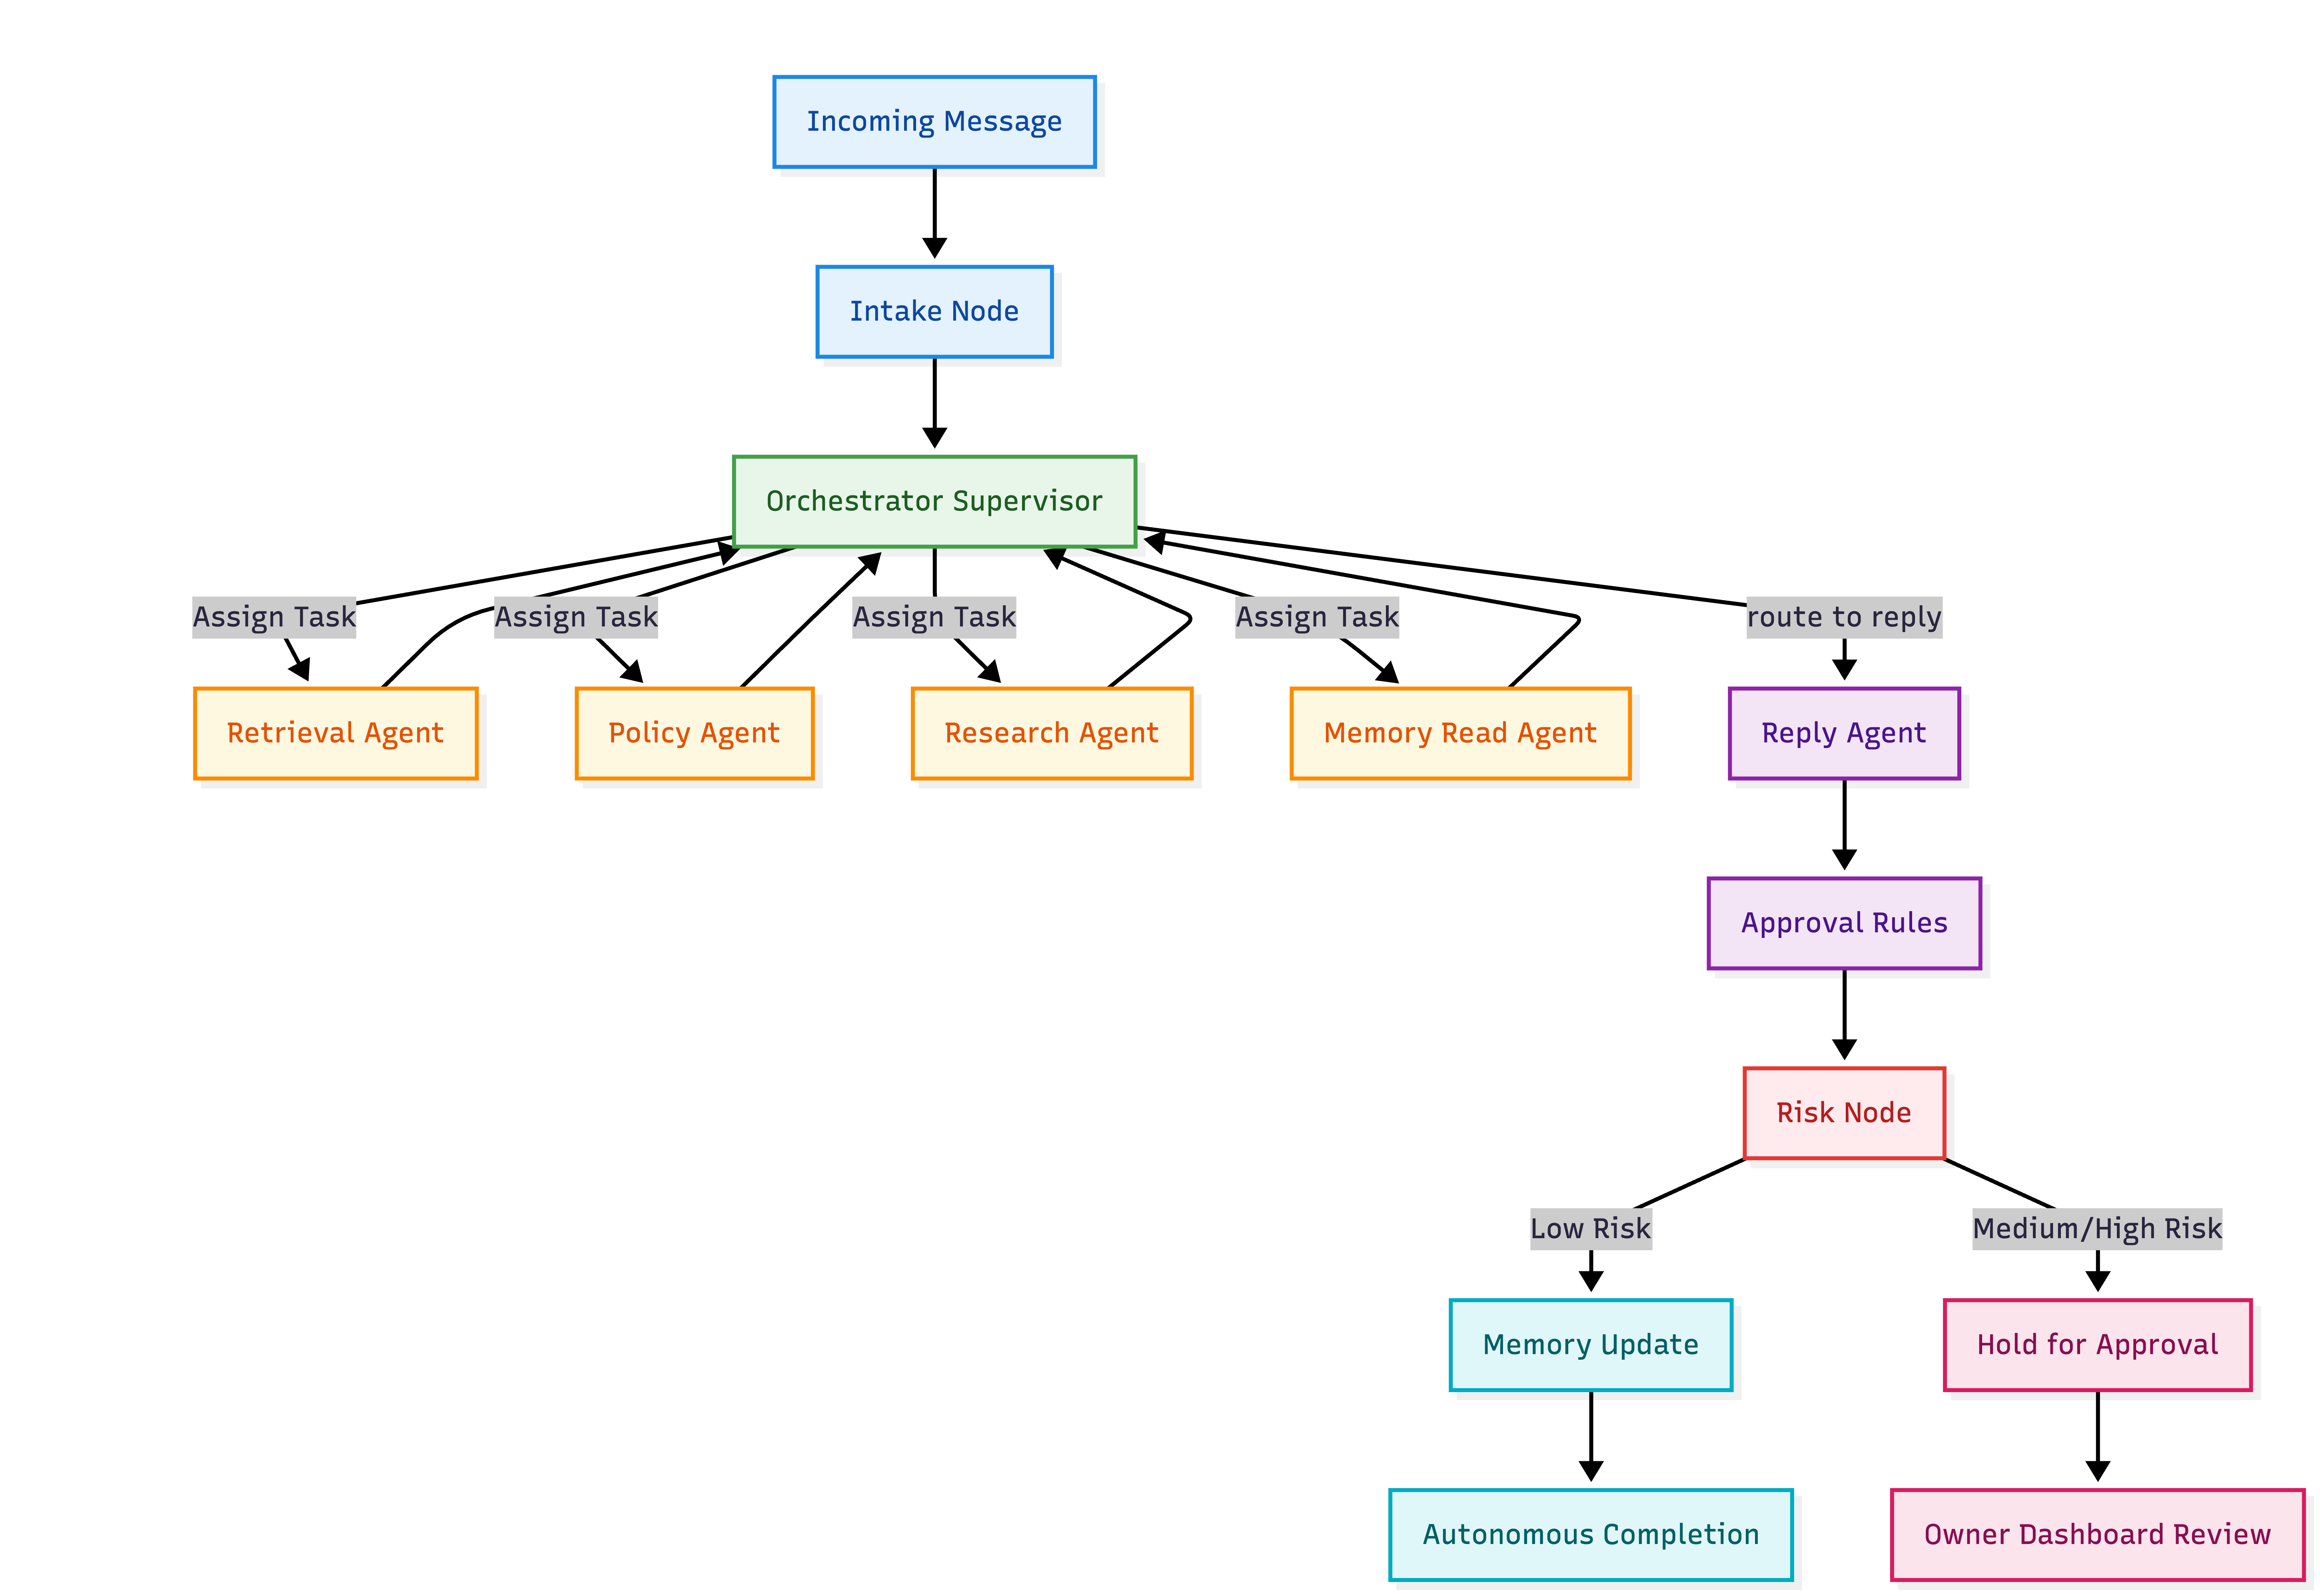
\includegraphics[width=0.8\textwidth]{mermaid.png}
    \caption{System Architecture and Flow}
    \label{fig:system-architecture}
\end{figure}

\subsection{Intake and Identity Resolution}
The intake node consolidates three formerly separate stages—receiver, triage, and context building—into a single efficient node. It resolves the sender's identity by normalizing external identifiers (email, phone, username) and querying the ExternalIdentity table. If the sender matches the owner's UUID or email, they are assigned the 'owner' role; otherwise, the system first attempts to match the sender against known mapped identities. If no prior mapping exists, the system conservatively creates the sender as a customer by default, avoiding unnecessary privilege escalation on first contact. The owner can later switch the stakeholder role in the dashboard, making this default a safe starting point rather than a permanent restriction. The node then loads owner-specific persona, rules, business description, and memory context from the database profile and memory services, and constructs the three-layer memory context: short-term chat history, durable long-term summaries, and sender-specific profile data. If profile fields are empty, the code falls back to conservative built-in default strings rather than reading local markdown files.

\subsection{Decision-Theoretic Framing: Approximate MEU Control}
We retain a decision-theoretic interpretation of the system because it captures the operational trade-off that the architecture is designed to manage. In particular, the pipeline can be understood as an \textit{approximate maximum expected utility (MEU)} control policy. The system does not solve an explicit probabilistic optimization problem with a learned utility function. Instead, it encodes utility through workflow structure: fast autonomous dispatch is preferred when the evidence is sufficient and the estimated downside is low, whereas replies are slowed down and escalated when the expected cost of a mistaken action outweighs the benefit of speed.

In our setting, the main competing objectives are response quality, policy compliance, confidentiality, reputational protection, and latency. The action space is intentionally bounded: the orchestrator may replan only a limited number of times, parallel fan-out is capped, and the final autonomy choice is effectively to send, hold for review, or fail safe. Low-risk replies maximize operational efficiency by being auto-sent. Medium- and high-risk replies are held for approval because the expected downside of false commitments, inappropriate concessions, or sensitive disclosure is greater than the value of immediate automation. The two-layer risk evaluator, confidence signals from the reply agent, and workflow-level approval hold therefore act as an engineering approximation to MEU: they choose the highest-autonomy action that remains acceptable under the system's encoded risk tolerance without claiming formal optimality.

\subsection{Orchestrator: Task Decomposition and Planning}

The orchestrator functions as a supervisor that decomposes requests into subtasks and assigns them to specialized agents. For recurring cases such as discount requests, supplier terms, and policy questions, it uses deterministic task paths; for novel or complex requests, it produces an LLM-generated plan with assignees, dependencies, and required context. A key design principle is \textit{synthesis-over-delegation}: before issuing new work, the orchestrator must incorporate results from completed tasks into later task descriptions so that sub-agents receive concrete facts rather than vague instructions. Replanning is bounded by MAX\_REPLAN\_CYCLES (default 2), and parallel dispatch is capped at MAX\_PARALLEL\_TASKS (default 4) to preserve controllability and keep fan-in manageable.


\subsection{Sub-Agent Specialization}

Four specialized sub-agents handle distinct aspects of request processing:

\begin{itemize}
\item \textbf{Retrieval Agent:} Fetches internal business data with role-based access control. The agent dynamically binds only the tools permitted for the sender's role via a fixed role-to-tool map, and includes a dedicated \texttt{evaluate\_discount\_request} tool with quantity-tiered pricing and margin-floor enforcement (cost $\times$ 1.12).

\item \textbf{Policy Agent:} Implements a hybrid RAG pipeline for grounded policy evaluation through semantic search, lexical search, candidate merging, and cross-encoder reranking, returning a structured \texttt{PolicyDecision} with verdict, supporting rules, confidence, and hard-constraint annotation.

\item \textbf{Research Agent:} Conducts external web search via the Tavily API and synthesizes results into a structured \texttt{ResearchSummary} with findings, sources, confidence, and caveats.

\item \textbf{Memory Agent:} Retrieves recent, durable, and stale historical context and proposes structured memory updates for owner approval after reply generation.
\end{itemize}

\subsection{Reply Generation}
The reply agent synthesizes all sub-agent results, the persona profile (SOUL), business rules (RULE), long-term memory, and conversation history into a final stakeholder-facing response. SOUL shapes the owner's style and business posture, RULE captures non-negotiable constraints, and long-term context helps the system stay consistent with prior commitments and relationship history. The agent applies role-specific tone postures: polite and transparent for customers (never revealing cost data), firm and profit-focused for suppliers, promotional and growth-oriented for investors, and professionally balanced for partners. Importantly, SOUL is not a hidden prompt artifact but an explicit owner-authored control surface: it is visible, editable, and auditable, which makes stylistic control more transparent than relying entirely on model priors. The agent outputs a structured ReplyOutput including the reply text, confidence level, unverified claims, and tone flags. This does not remove the need for downstream human evaluation of usefulness or stakeholder acceptance, but it does make tone control substantially more inspectable and owner-governed.

\subsection{Two-Layer Risk Evaluation}

All outgoing replies undergo a two-layer risk evaluation before dispatch:

\textbf{Layer 1 — Rule-Based (Deterministic):} A comprehensive set of regex-based detectors checks for: price commitments, delivery guarantees, escalation triggers (lawsuit, breach, recall), confidentiality violations (margin/cost disclosure), PII leakage (credit card numbers, SSNs, API keys), role-based sensitivity violations, policy cross-checks, unverified claims, low-confidence signals, and tone anomalies. Escalation triggers and PII leaks immediately escalate to HIGH risk; multiple flag categories yield MEDIUM; minor flags yield LOW.

\textbf{Layer 2 — LLM Semantic Analysis:} Triggered only for MEDIUM-risk results from Layer 1, this layer uses an LLM (gpt-4o-mini at temperature 0.0) to detect implied commitments, factual contradictions with sub-agent findings, contextual liability, intent mismatches, and nuanced tone issues. The LLM can upgrade or downgrade the risk level and add semantic flags. If the LLM call fails, the system gracefully falls back to the Layer 1 assessment.

\subsection{Approval Workflow}

Replies assessed as MEDIUM or HIGH risk are held for owner approval. The hold\_for\_approval node persists the draft reply to the held\_replies table and creates a pending\_approvals entry visible on the owner dashboard. The owner can approve (triggering message dispatch) or reject (with an optional reason). All decisions are recorded in reply\_review\_records for audit purposes. Owner-originated messages bypass both approval rules and risk evaluation. An example end-to-end walkthrough of a discount request is provided in Appendix~\ref{app:walkthrough}.

\section{Implementation}

The implementation combines a FastAPI backend, a LangGraph state graph, Supabase/PostgreSQL storage with Row-Level Security, and a Next.js frontend. The database is organized around core entities, products and orders, policy chunks, memory, and approval records, while the live system is exposed through message-ingestion and approval endpoints used by the owner dashboard. At runtime, the graph follows the topology intake $\rightarrow$ orchestrator $\rightarrow$ conditional fan-out to sub-agents $\rightarrow$ reply $\rightarrow$ approval rules $\rightarrow$ risk $\rightarrow$ auto-send or hold-for-approval. Detailed stack, schema, full architecture, and code-availability materials are provided in Appendix~\ref{app:techstack}, Appendix~\ref{app:schema}, Appendix~\ref{appendix:architecture}, and Appendix~\ref{app:repo}.

Several implementation choices are especially important to the paper's claims. All agents emit Pydantic-validated outputs so downstream nodes receive typed state rather than free-form text. To preserve controllability under failure, the pipeline uses bounded replanning, capped parallelism, task-budget guards, error quarantine, and context-compression circuit breakers; failures are converted into structured task artifacts rather than crashing the graph, and internal stack traces are sanitized before later nodes or users see them.

Security and review are also enforced in infrastructure rather than prompts. RBAC is implemented at the retrieval tool-binding layer through a fixed role-to-tool map, creating a hard boundary independent of prompt compliance. The approval path persists held drafts, pending approvals, and review records for owner decisions, while the frontend provides the live interface through which the owner reviews replies and memory proposals.

\section{Results and Analysis}
\subsection{Evaluation Design}

The evaluation is organized around the paper's core principles: human collaboration, role-aware control, grounded reasoning, transparency, responsible behavior, and operational performance.

\begin{itemize}
\item \textbf{D1 Human collaboration and oversight:} Does the system preserve owner control over high-stakes commitments while reducing low-risk manual effort?
\item \textbf{D2 Role awareness and access control:} Does the pipeline treat stakeholder roles appropriately and enforce confidentiality boundaries through RBAC and identity resolution?
\item \textbf{D3 Grounded policy reasoning:} Does the policy path retrieve relevant evidence, identify hard constraints, and tie decisions to business rules?
\item \textbf{D4 Observability and workflow guarantees:} Are intermediate decisions inspectable and consistent with the intended auto-send, hold-for-approval, fan-out/fan-in, and failure-quarantine behavior?
\item \textbf{D5 Fairness and responsible AI behavior:} Are role-based differences explicit and auditable, with unknown senders and sensitive data handled by transparent rules?
\item \textbf{D6 Operational usefulness:} Does the system achieve acceptable accuracy, latency, and bounded autonomy for deployment-oriented business communication?
\end{itemize}

To evaluate these dimensions, we combine three evidence sources: ground-truth policy benchmarking, deterministic test suites for safety- and control-critical logic, and mocked end-to-end pipeline integration tests. This mirrors the system's division of responsibility: the AI handles grounded retrieval, policy interpretation, synthesis, and low-risk drafting, while the owner retains authority over high-risk commitments, exceptions, and sensitive disclosures. Reproducible workflow checks therefore serve as the primary evidence for controllability.

One further nuance is that stylistic control is handled partly by design rather than evaluation alone. Because SOUL is explicit, owner-authored, and editable, tone alignment is more transparent than hidden prompt steering and easier for the owner to govern directly.

\subsection{Main Quantitative Results}

The strongest quantitative evidence is on the policy path. On the committed 44-query benchmark, the policy agent achieved 90.9\% overall verdict accuracy, 100.0\% hard-constraint detection, a 2.6\% false \texttt{not\_covered} rate, and a 0.0\% hallucinated-supporting-rule rate under our overlap-based faithfulness proxy. Across selected deterministic suites, 104 tests passed with 2 skipped, covering identity resolution, approval rules, risk logic, discount negotiation behavior, and mocked end-to-end pipeline flows. Together these results support a bounded claim of controllable, policy-grounded autonomy rather than blanket end-to-end superiority over simpler alternatives. Appendix~\ref{app:eval-extended} and Appendix~\ref{app:eval-coverage} provide fuller tables and plots.

\subsection{Performance and Trade-offs}

Several architectural trade-offs are visible in the current evidence:
\begin{itemize}\itemsep0.15em \parsep0pt \topsep0.25em \partopsep0pt
\item \textbf{RAG quality vs. latency:} Grounded policy reasoning improves traceability and decision quality, but mean and p95 policy-path latency are 3414.7 ms and 4358.4 ms.
\item \textbf{Risk coverage vs. simplicity:} The two-layer risk design adds complexity, but keeps explicit cases cheap while reserving LLM review for ambiguity.
\item \textbf{Parallelism vs. controllability:} LangGraph fan-out improves modularity and throughput, but capped parallelism and bounded replanning remain necessary to control cost and state growth.
\item \textbf{Automation vs. owner control:} The approximate MEU policy is intentionally conservative, trading immediacy for bounded downside on high-stakes replies.
\end{itemize}
\noindent
The current evaluation is centered on policy grounding and control-flow behavior. Matched single-agent comparison, broader live interaction studies, and larger category coverage are natural extensions of this evaluation scope, while the approximate MEU framing remains an interpretive lens rather than a formal optimality result. Appendix~\ref{app:eval-validity} provides the extended validity discussion and baseline design.
\section{Fairness, Responsibility \& Ethics}

\subsection{Bias and Fairness Considerations}

Several sources of bias warrant consideration:

\begin{itemize}
\item \textbf{Model and retrieval bias:} The system relies on GPT-4o-mini and Gemini, which inherit biases from training data, and on a hybrid RAG pipeline whose behavior depends on policy coverage and embedding quality. Together, these components may affect task planning, tone generation, information synthesis, and whether valid queries are treated as sufficiently covered.

\item \textbf{Role-based asymmetry and correction latency:} The system deliberately enforces different access levels and communication styles by stakeholder role. Unknown inbound senders are conservatively initialized as customers when no prior identity mapping exists, which minimizes overexposure of privileged data but makes fairness dependent on low correction latency if a sender is later confirmed to be a supplier, partner, or investor.

\item \textbf{Procedural fairness in negotiation and risk review:} The evaluate\_discount\_request tool applies fixed quantity-based pricing rules, which improves consistency but ignores factors such as customer loyalty or relationship history. More broadly, fairness in this system also requires similar requests to receive comparable response quality, policy treatment, and risk flagging, without disproportionate penalties for linguistic style or background.
\end{itemize}

Several design choices reduce the risk of arbitrary or judgmental behaviour. The system does not make demographic inference a first-class decision variable; instead, it relies on explicit role mappings, owner-authored constraints, and verified relationship history. Fairness in this setting is therefore procedural as well as representational: role-based differentiation should remain justified and auditable, newly discovered stakeholders should be corrected quickly, and equivalent requests should not receive inconsistent negotiation or risk treatment for irrelevant reasons.

\subsection{Implemented Responsible-AI Safeguards}

The system already incorporates several responsible-AI mechanisms in the implemented workflow:

\begin{itemize}
\item \textbf{Human oversight and accountability:} No reply assessed as MEDIUM or HIGH risk is dispatched without explicit owner review. This makes human control operational rather than merely advisory\textsuperscript{[20,23]}.

\item \textbf{Owner-guided and traceable behavior:} Reply generation is conditioned on owner-authored SOUL identity, RULE constraints, and long-term memory context. Because SOUL is explicit and editable, tone control is more transparent and owner-governed than if style were left entirely to hidden prompt settings or model priors.

\item \textbf{Workflow-level governance:} Role-scoped tool binding, structured outputs, bounded replanning, token-budget guards, error quarantine, and fallback behavior ensure that responsibility is implemented at the harness level rather than delegated entirely to prompt compliance.

\item \textbf{Security-aware design:} Tool-level RBAC directly addresses the practical risk that prompt injection can subvert prompt-level restrictions\textsuperscript{[21,22]}.
\end{itemize}

\subsection{Residual Ethical Risks and Future Mitigations}

Even with these safeguards, several ethical risks remain open:

\begin{itemize}
\item \textbf{Transparency of AI involvement:} The system can generate replies on behalf of the owner, so users should be informed when they are interacting with AI-assisted communication. A stronger production version should support mandatory disclosure templates.

\item \textbf{Manipulative communication risk:} Because the system is designed to persuade, negotiate, and maintain relationships, it could produce overly forceful or strategically manipulative language. Extending tone analysis toward persuasion-risk detection would strengthen governance.

\item \textbf{Privacy and retention obligations:} The system stores conversations, sender profiles, and memory summaries. A production deployment therefore requires retention limits, deletion workflows, and stronger compliance handling for personal data.

\item \textbf{Prompt injection and indirect influence:} Adversarial or retrieved content may still attempt to manipulate downstream reasoning. RBAC and risk review reduce this risk, but they do not eliminate it\textsuperscript{[21,22]}.
\end{itemize}


\section{Extensibility \& Future Work}

\subsection{Extensibility and Scalability}
The architecture is designed to grow without rewriting the core pipeline. New agents can be added as LangGraph nodes, new roles by extending ROLE\_TOOL\_MAP and the data model, and new policy corpora through ingestion rather than pipeline changes. Supabase with RLS, LangGraph fan-out, pgvector with HNSW indexing, and token budgeting with memory compaction provide the main scalability hooks.

\subsection{Future Directions}

The most important next steps are a fair matched baseline against a strong single-agent assistant, live end-to-end and human evaluation, tighter calibration of the approximate MEU escalation policy, and broader channel and model support.

\section{Conclusion}

This report presented a multi-agent orchestration system for managing business communication in solo enterprises. Its contribution is hybrid: as an application paper, it combines role-aware retrieval, policy grounding, memory, and approval-gated reply generation into a practical communication-management system; as a methodological paper, it argues that safety-critical behavior can be moved out of prompts and into workflow structure, turning autonomy into a more controllable and reviewable decision policy.

The current evidence supports three bounded claims. The policy path is meaningfully grounded: on a 44-query benchmark it achieved 90.9\% verdict accuracy and 100.0\% hard-constraint detection. The deterministic control layer is also well covered, with 104 passing tests across selected safety and control-flow suites. Finally, the architecture supports a plausible approximate MEU interpretation for trust-sensitive communication by allowing autonomy where the expected downside is low and escalating where the expected cost of error is high.

The paper should also be read in line with its current emphasis. The empirical story centers on policy evaluation and workflow guarantees, while future extensions can broaden this with richer human-centered assessment, live production studies, matched baseline experiments, and further calibration of the autonomy-versus-escalation policy.
\clearpage

\begin{thebibliography}{15}

\bibitem{1}
Wooldridge M. An Introduction to MultiAgent Systems. 2nd ed. Chichester: John Wiley \& Sons; 2009.

\bibitem{2}
Wu Q, Bansal G, Zhang J, Wu Y, Li B, Zhu E, et al. AutoGen: Enabling Next-Gen LLM applications via Multi-Agent Conversation [Internet]. arXiv.org. 2023. Available from: https://arxiv.org/abs/2308.08155

\bibitem{3}
CrewAI. CrewAI: Framework for orchestrating role-playing AI agents [Internet]. 2024 [cited 2026 Apr 16]. Available from: https://github.com/crewAIInc/crewAI

\bibitem{4}
LangChain. LangGraph: Build resilient language agents as graphs [Internet]. 2024 [cited 2026 Apr 16]. Available from: https://github.com/langchain-ai/langgraph

\bibitem{5}
Nau D, Au TC, Ilghami O, Kuter U, Murdock JW, Wu D, et al. SHOP2: An HTN planning system. J Artif Intell Res. 2003;20:379–404.

\bibitem{6}
Lewis P, Perez E, Piktus A, Petroni F, Karpukhin V, Goyal N, et al. Retrieval-Augmented Generation for Knowledge-Intensive NLP Tasks. Adv Neural Inf Process Syst. 2020;33:9459-74.

\bibitem{7}
Ma X, Gong Y, He P, Zhao H, Duan N. Query rewriting for Retrieval-Augmented Large Language Models [Internet]. arXiv.org. 2023. Available from: https://arxiv.org/abs/2305.14283

\bibitem{8}
Nogueira R, Jiang Z, Pradeep R, Lin J. Document ranking with a pretrained sequence-to-sequence model. In: Findings of EMNLP; 2020. p. 708–18.

\bibitem{9}
Li X, Zhang Y, Stolfo A. mixedbread-ai/mxbai-rerank-base-v1 [Internet]. Hugging Face; 2024 [cited 2026 Apr 16]. Available from: https://huggingface.co/mixedbread-ai/mxbai-rerank-base-v1

\bibitem{10}
NVIDIA. NeMo Guardrails: A Toolkit for Controllable and Safe LLM Applications with Programmable Rails [Internet]. 2023 [cited 2026 Apr 16]. Available from: https://github.com/NVIDIA/NeMo-Guardrails

\bibitem{11}
Guardrails AI. Guardrails: Adding guardrails to large language models [Internet]. 2024 [cited 2026 Apr 16]. Available from: https://github.com/guardrails-ai/guardrails

\bibitem{12}
National Security Agency. \textit{Defense in Depth: A Practical Strategy for Achieving Information Assurance in Today's Highly Networked Environments} [Internet]. Available from: https://www.nsa.gov/ia/\_files/support/defenseindepth.pdf

\bibitem{13}
Sandhu RS, Coyne EJ, Feinstein HL, Youman CE. Role-Based Access Control Models. IEEE Comput. 1996;29(2):38–47.

\bibitem{14}
Park JS, O'Brien J, Cai CJ, Morris MR, Liang P, Bernstein MS. Generative agents: Interactive simulacra of human behavior. InProceedings of the 36th annual acm symposium on user interface software and technology 2023 Oct 29 (pp. 1-22).

\bibitem{15}
Packer C, Wooders S, Lin K, Fang V, Patil SG, Stoica I, et al. MemGPT: Towards LLMs as Operating Systems [Internet]. arXiv.org. 2023. Available from: https://arxiv.org/abs/2310.08560

\bibitem{16}
Wang L, Ma C, Feng X, Zhang Z, Yang H, Zhang J, et al. A survey on large language model based autonomous agents. Front Comput Sci. 2024;18:186345.

\bibitem{17}
Gao Y, Xiong Y, Gao X, Jia K, Pan J, Bi Y, et al. Retrieval-Augmented Generation for Large Language Models: A Survey [Internet]. arXiv.org. 2023. Available from: https://arxiv.org/abs/2312.10997

\bibitem{18}
Chen J, Lin H, Han X, Sun L. Benchmarking Large Language Models in Retrieval-Augmented Generation. Proc AAAI Conf Artif Intell. 2024;38(16):17754--17762.

\bibitem{19}
Es S, James J, Espinosa-Anke L, Schockaert S. RAGAs: Automated Evaluation of Retrieval Augmented Generation. In: Proceedings of the 18th Conference of the European Chapter of the Association for Computational Linguistics: System Demonstrations; 2024. p. 150--158.

\bibitem{20}
Amershi S, Weld D, Vorvoreanu M, Fourney A, Nushi B, Collisson P, et al. Guidelines for Human-AI Interaction. In: Proceedings of the 2019 CHI Conference on Human Factors in Computing Systems; 2019. p. 1--13.

\bibitem{21}
Perez F, Ribeiro I. Ignore Previous Prompt: Attack Techniques for Language Models [Internet]. arXiv.org. 2022. Available from: https://arxiv.org/abs/2211.09527

\bibitem{22}
Greshake K, Abdelnabi S, Mishra S, Endres C, Holz T, Fritz M. Not what you've signed up for: Compromising Real-World LLM-Integrated Applications with Indirect Prompt Injection [Internet]. arXiv.org. 2023. Available from: https://arxiv.org/abs/2302.12173

\bibitem{23}
Shneiderman B. Human-Centered Artificial Intelligence: Reliable, Safe \& Trustworthy. Int J Hum Comput Interact. 2020;36(6):495--504.

\end{thebibliography}

\clearpage
\appendix
\section{Appendix}
\label{sec:appendix}
\addcontentsline{toc}{section}{Appendix} % optional (for TOC)

\subsection{Architecture Control Boundaries}
\label{app:control-table}

\renewcommand{\arraystretch}{1.25}
\begin{tabular}{|p{2.0cm}|p{3.0cm}|p{3.4cm}|p{4.8cm}|}
\hline
\textbf{Stage} & \textbf{Primary function} & \textbf{Deterministic controls} & \textbf{Main output} \\
\hline
Intake & Resolve sender identity, assign a conservative role, and load persona, rules, and memory context. & Unknown senders default to customer role; identity is normalized against the external\_identities mapping before any privileged retrieval occurs. & Role assignment plus a shared state seeded with owner profile, memory context, and conversation metadata. \\
\hline
Orchestrator & Decompose the message into sub-tasks and schedule specialized agents. & Deterministic fast paths for common cases, capped parallel fan-out, and bounded replanning cycles. & A task plan that specifies which agents are invoked and what evidence each agent must return. \\
\hline
Specialized agents & Retrieve internal data, evaluate policy, run external research, and recover relevant memory. & RBAC is enforced at tool-binding time; policy outputs are structured and grounded; failures are quarantined rather than silently merged. & Typed evidence artifacts such as retrieval results, policy decisions, research summaries, and memory summaries. \\
\hline
Reply generation & Synthesize a stakeholder-facing draft from the accumulated evidence and owner-authored context. & Pydantic-validated structured output, explicit confidence fields, and flags for unverifiable claims or tone issues. & A draft reply paired with metadata used by downstream approval and risk nodes. \\
\hline
Approval and risk & Decide whether the reply can be auto-sent or must be held for owner review. & Deterministic approval rules, regex-based risk checks, optional LLM semantic escalation, and persistent review records. & Either automatic dispatch for low-risk messages or a held draft awaiting owner approval. \\
\hline
\end{tabular}

\subsection{Example End-to-End Walkthrough}
\label{app:walkthrough}

The walkthrough below makes the control flow concrete for the reader.

\begin{enumerate}
\item A customer asks whether a bulk order of 200 units can receive a 15\% discount and next-week delivery. The intake node resolves the sender as a customer, loads the owner's SOUL and RULE context, and recovers recent conversation memory.
\item The orchestrator recognizes a discount-negotiation pattern and dispatches the retrieval and policy agents in parallel. Retrieval checks product data, current quantity-tier rules, and the configured margin floor. The policy agent searches the business policy store for any rules related to pricing commitments and delivery promises.
\item The retrieval agent returns a structured discount evaluation showing whether the requested concession violates the configured minimum margin. In parallel, the policy agent returns a grounded verdict stating whether the reply may promise price or delivery terms without owner approval.
\item The reply agent synthesizes these results into a draft that stays within the approved pricing envelope and avoids unsupported delivery guarantees. It also exposes confidence and any unverified-claim flags in structured metadata.
\item The approval and risk stages then determine the autonomy level. If the reply stays within approved discount tiers and avoids risky commitments, it can be auto-sent. If it includes an exception, aggressive concession, or delivery promise, the draft is persisted and held for owner review.
\end{enumerate}

\subsection{Extended Evaluation Summary}
\label{app:eval-extended}

Table~\ref{tab:appendix-eval-summary} consolidates the main evaluation signals used in the paper. These results combine the committed policy benchmark with deterministic safety and integration suites.

\begin{table}[H]
\centering
\renewcommand{\arraystretch}{1.2}
\begin{tabular}{|p{3.0cm}|p{2.2cm}|p{3.0cm}|p{4.5cm}|}
\hline
\textbf{Artifact} & \textbf{Scope} & \textbf{Key result} & \textbf{Interpretation} \\
\hline
Policy verdict benchmark & 44 policy queries & 90.9\% overall verdict accuracy & The policy path is usually correct about whether a request is allowed, disallowed, or not covered. \\
\hline
Hard-constraint detection & 44 policy queries & 100.0\% detection rate & The benchmark did not contain any missed hard denials, which is important for safety-critical policy constraints. \\
\hline
Faithfulness proxy & 44 policy queries & 0.0\% hallucinated supporting rules & Retrieved evidence overlaps with the cited support in the current benchmark, though this remains a proxy rather than a full human audit. \\
\hline
Policy-path latency & 44 policy queries & 3414.7 ms mean, 4358.4 ms p95 & Hybrid retrieval and reranking improve grounding at a visible runtime cost. \\
\hline
Deterministic safety suites & Selected unit and integration suites & 104 passed, 2 skipped & Identity resolution, approval rules, risk checks, discount logic, and pipeline guarantees behaved as expected in the current test set. \\
\hline
Pipeline integration tests & 4 mocked end-to-end scenarios & 4 passed & The graph preserved low-risk auto-send, hold-for-approval, fan-out/fan-in aggregation, and failure quarantine in mocked end-to-end flows. \\
\hline
\end{tabular}
\caption{Extended evaluation summary used by the main paper.}
\label{tab:appendix-eval-summary}
\end{table}

\begin{figure}[H]
    \centering
    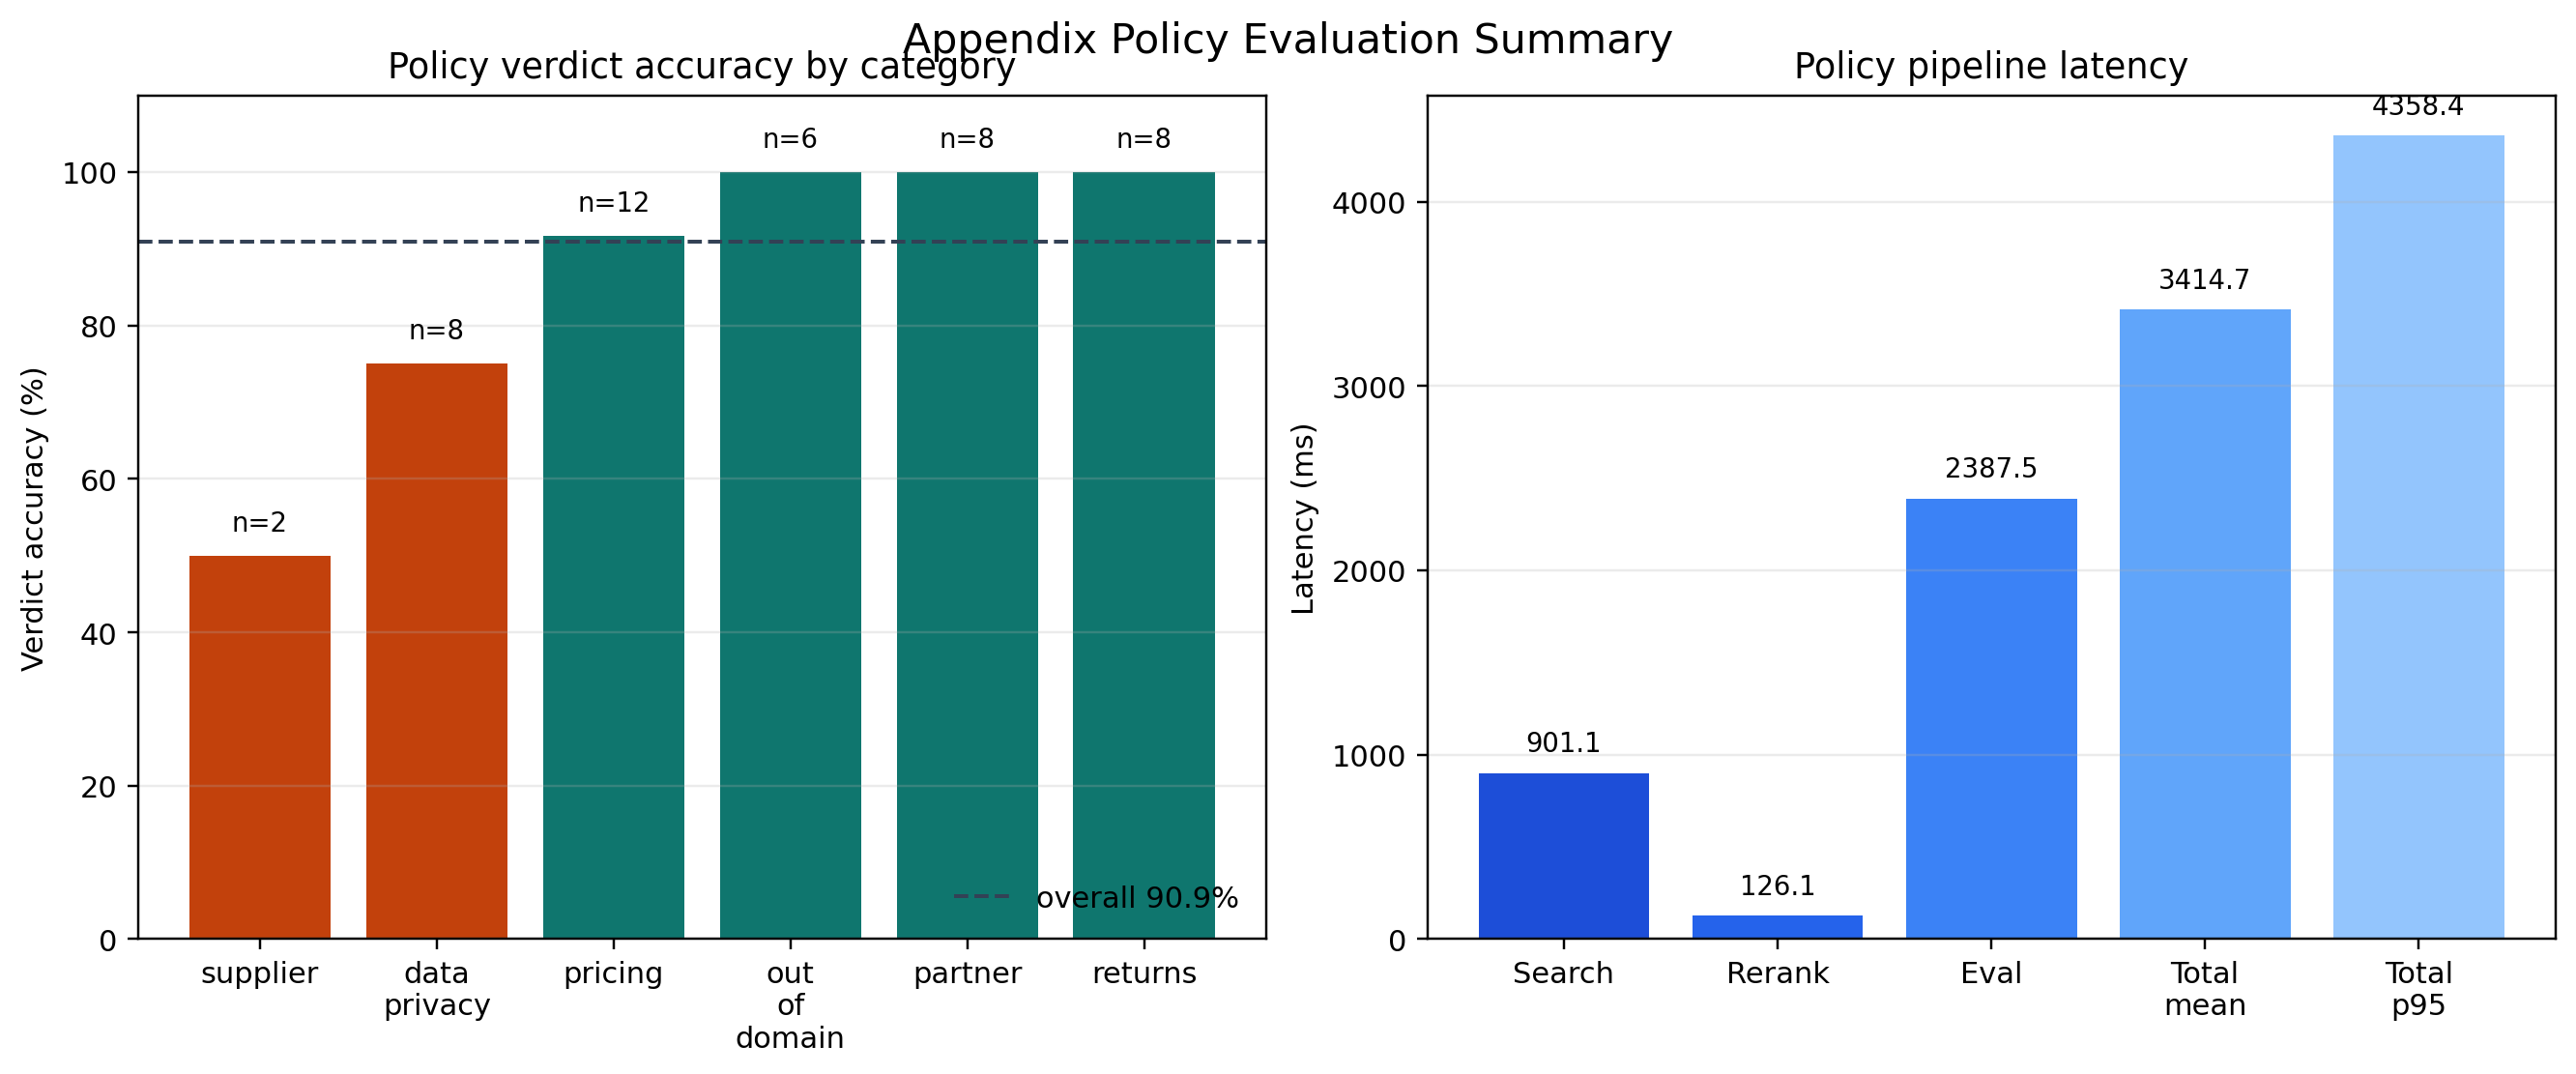
\includegraphics[width=0.96\textwidth]{appendix_policy_eval_summary.png}
    \caption{Policy benchmark summary generated from the committed evaluation artifact \texttt{tests/policy\_agent/results/answer\_metrics.json}. Left: category-level verdict accuracy with sample counts. Right: mean latency by policy-pipeline stage and total-path p95 latency.}
    \label{fig:appendix-policy-eval-summary}
\end{figure}

\paragraph{Failure analysis.}
The current benchmark indicates that the policy path is strongest on out-of-domain, partner, and returns queries, while data-privacy and supplier cases remain the most informative areas for further expansion. In particular, data-privacy queries reached 75.0\% verdict accuracy over 8 samples, and supplier queries reached 50.0\% over 2 samples. These slices are best read as directional signals that highlight where broader policy coverage and expanded evaluation would be most valuable.

\paragraph{Evaluation scope.}
The empirical story is anchored most strongly in grounded policy evaluation and deterministic workflow guarantees. The pipeline integration tests are intentionally mocked so that control-flow guarantees are isolated and reproducible, and they complement future live end-to-end studies with real channels, real owners, and real stakeholders.

\paragraph{Additional diagnostic figures.}
The figures below provide more granular agent-level evaluation artifacts complementing the summary table and policy benchmark plot above.

\begin{figure}[H]
    \centering
    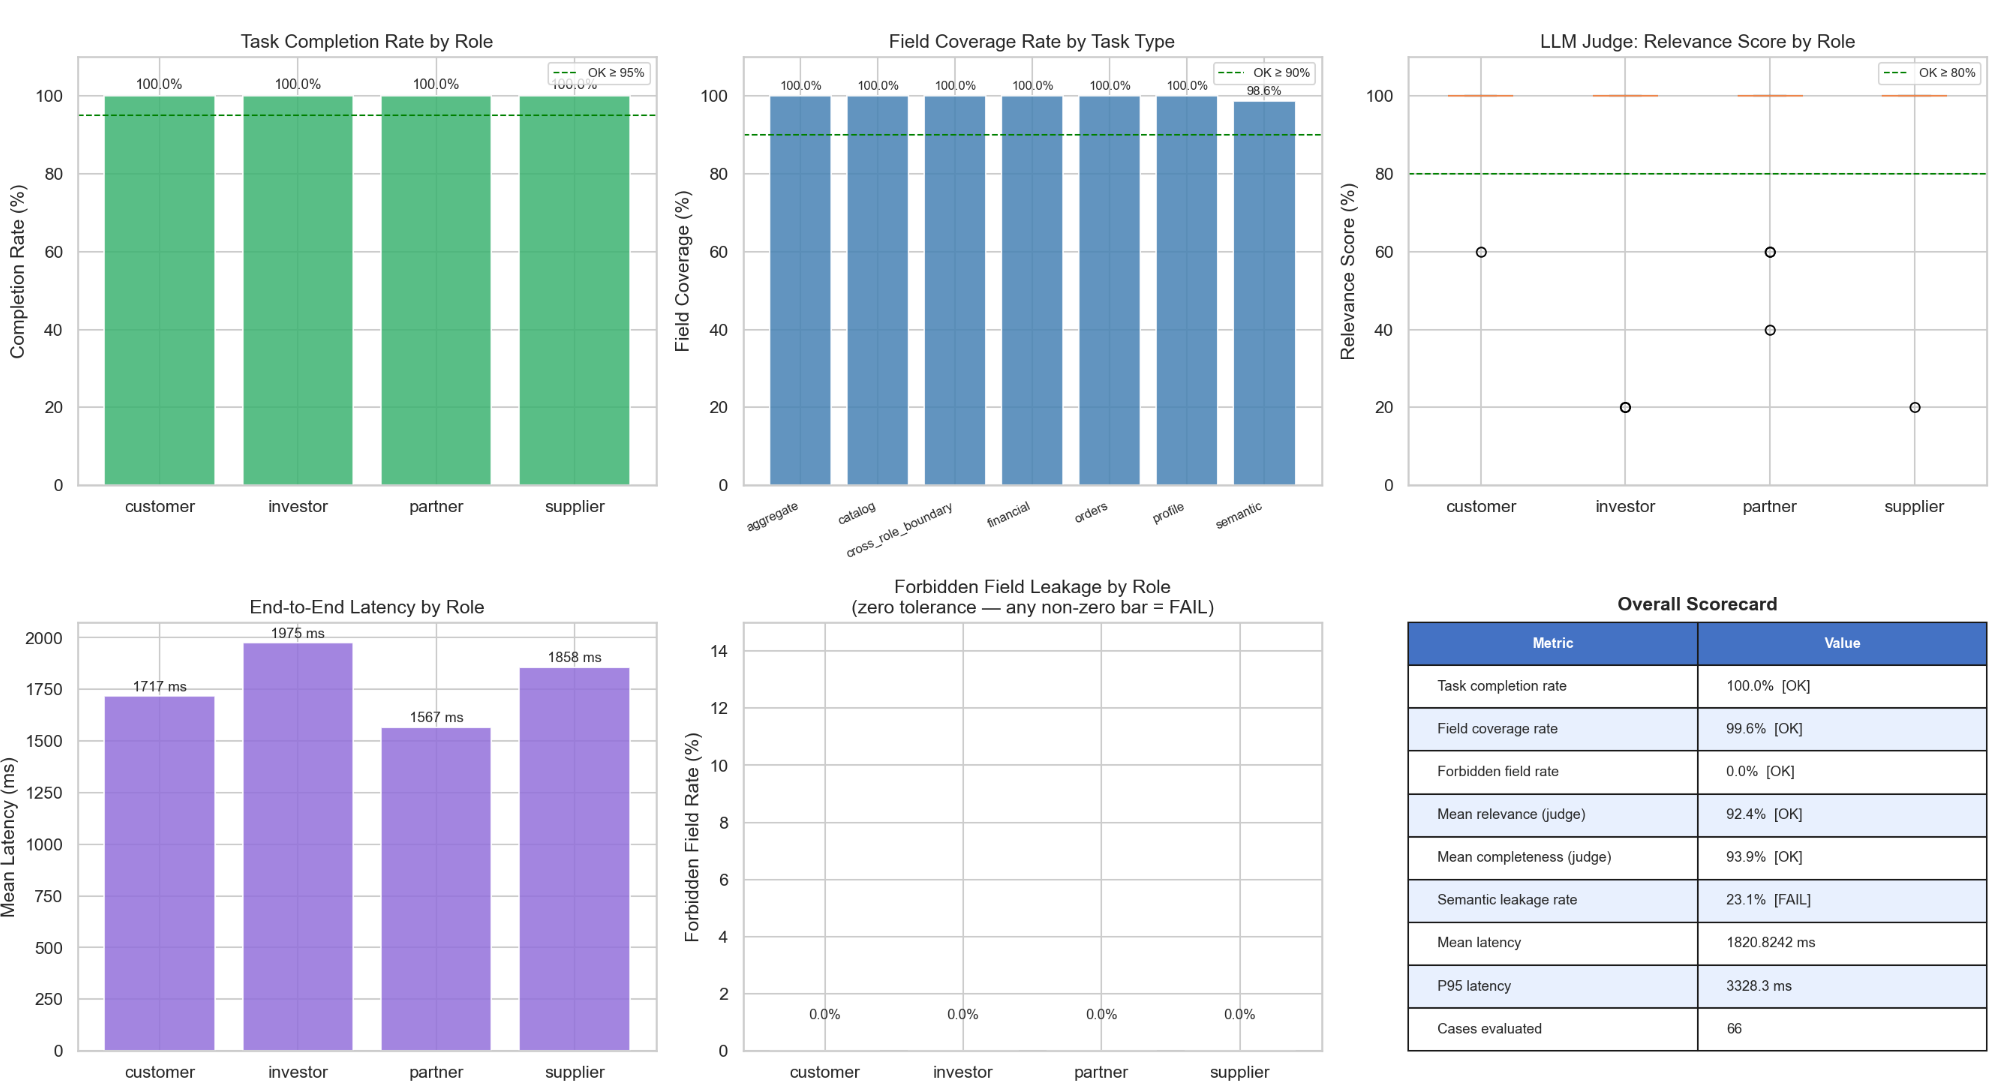
\includegraphics[width=0.8\textwidth]{fig1.png}
    \caption{Metrics for DB search in Retrieval Agent}
    \label{fig:retrieval-metrics}
\end{figure}
\begin{figure}[H]
    \centering
    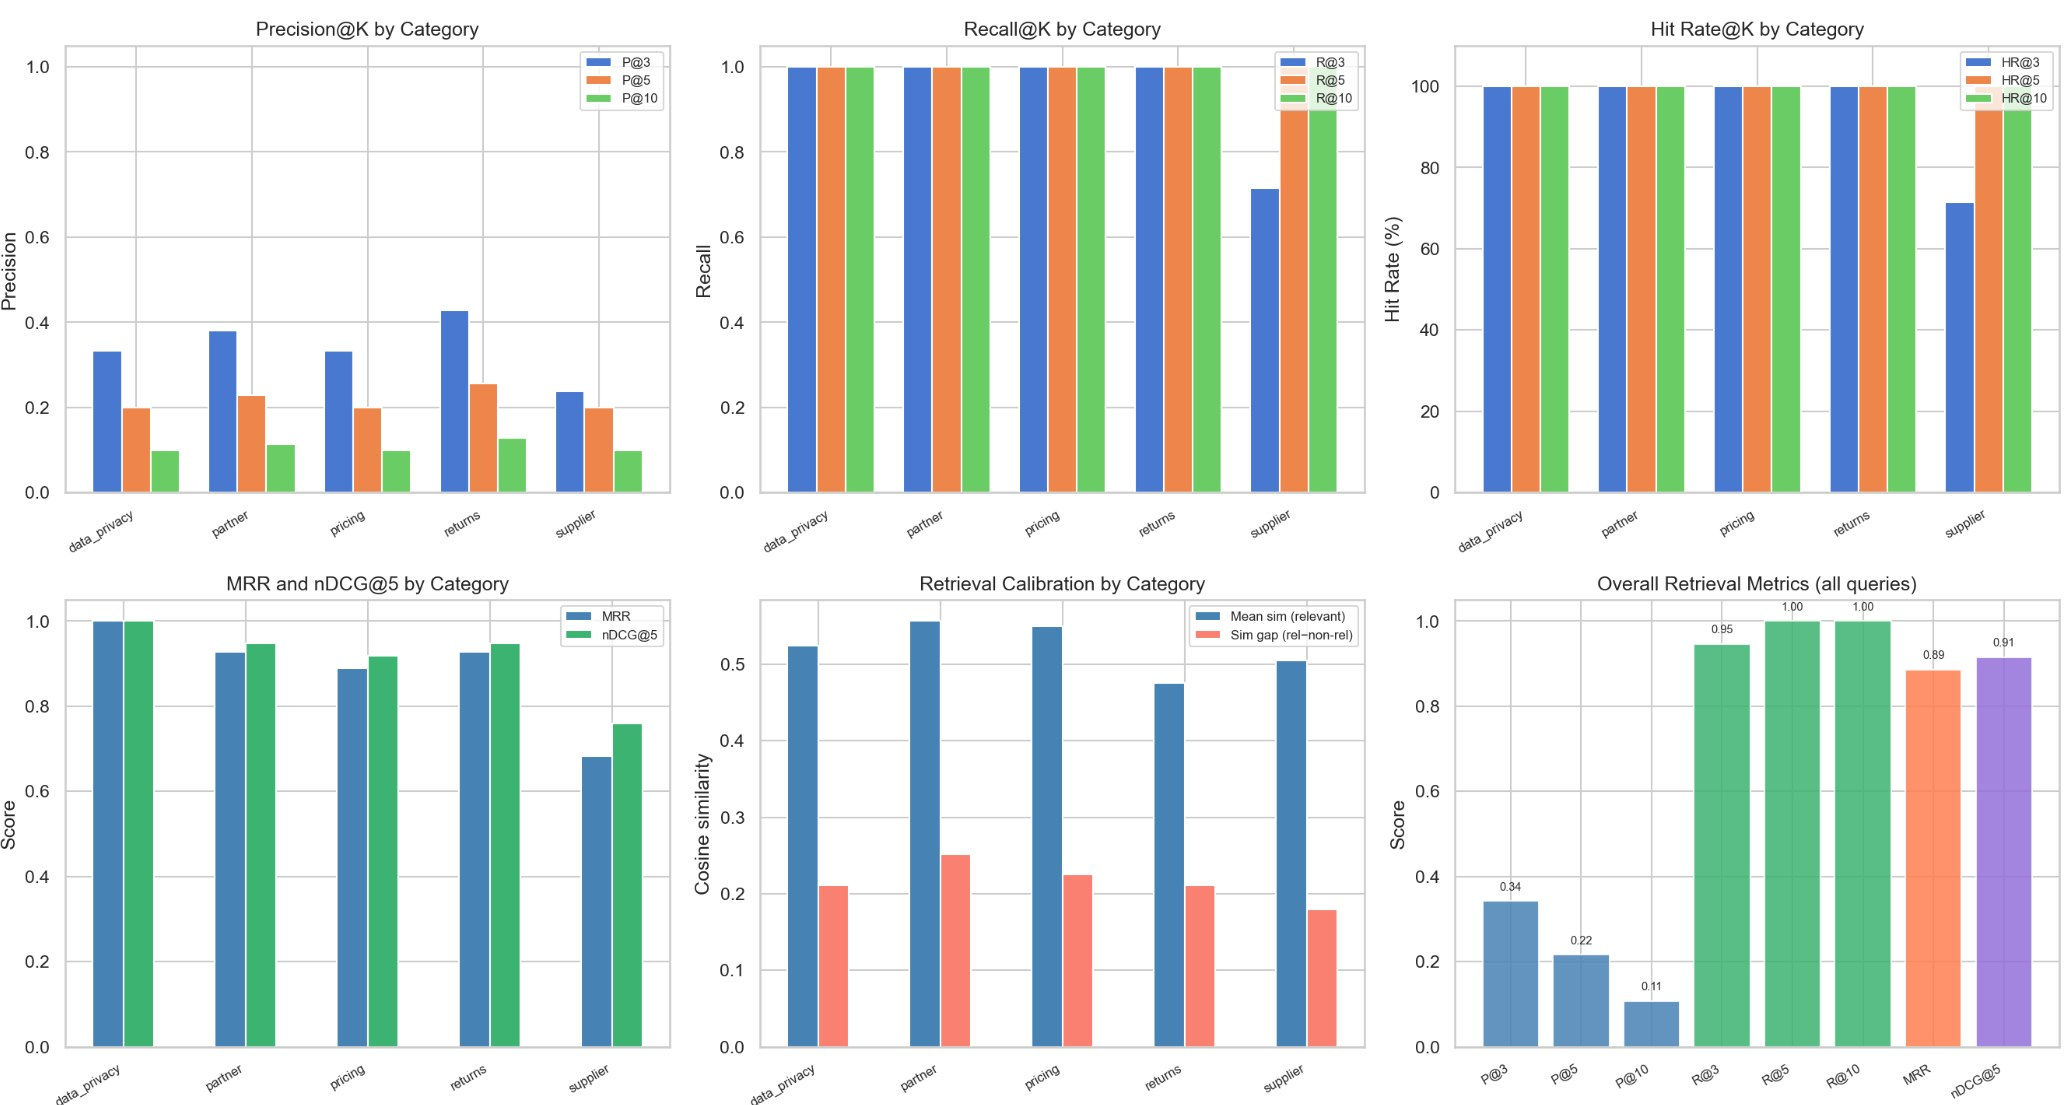
\includegraphics[width=0.8\textwidth]{fig2.jpg}
    \caption{Metrics for RAG in Policy Agent}
    \label{fig:policy-rag-metrics}
\end{figure}
\begin{figure}[H]
    \centering
    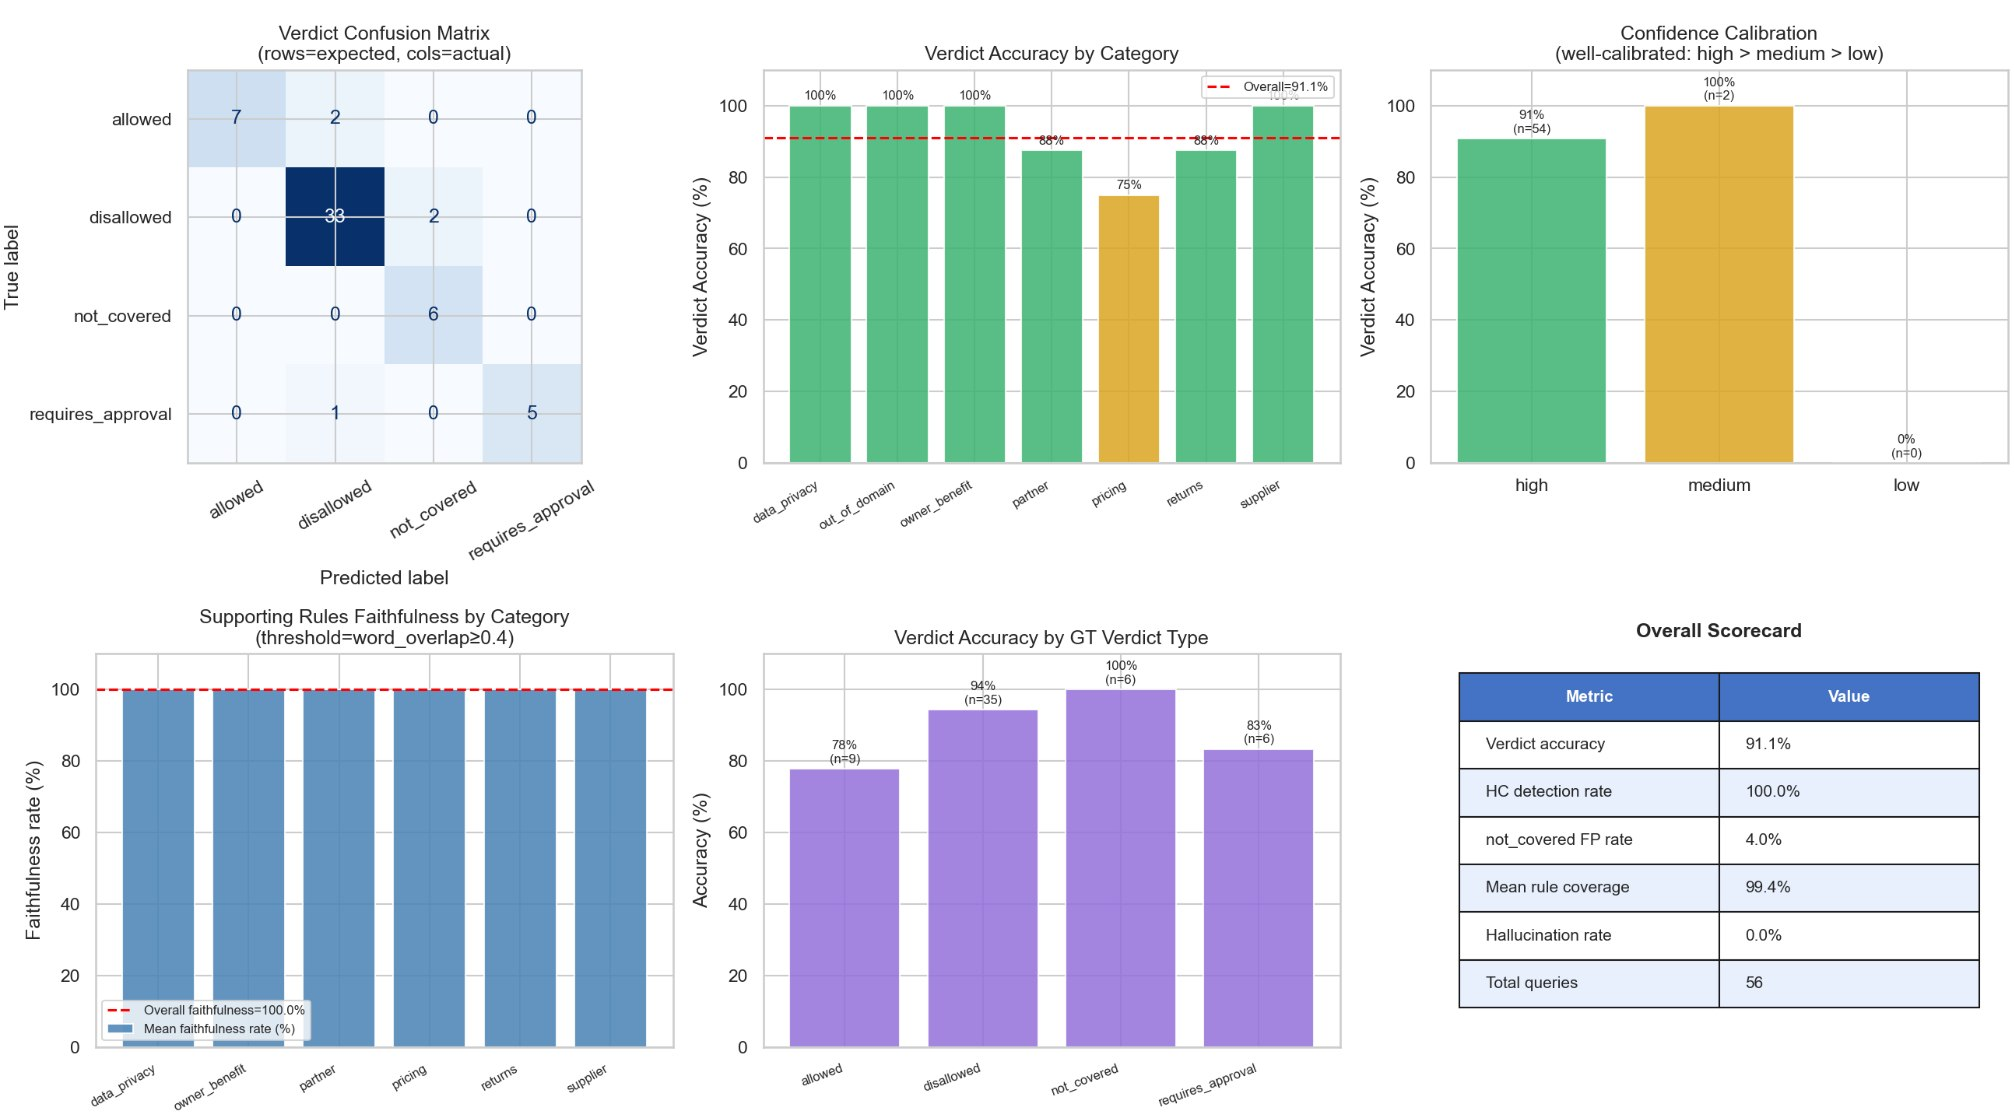
\includegraphics[width=0.8\textwidth]{fig3.jpg}
    \caption{Metrics for Policy Decisions in Policy Agent}
    \label{fig:policy-decision-metrics}
\end{figure}
\begin{figure}[H]
    \centering
    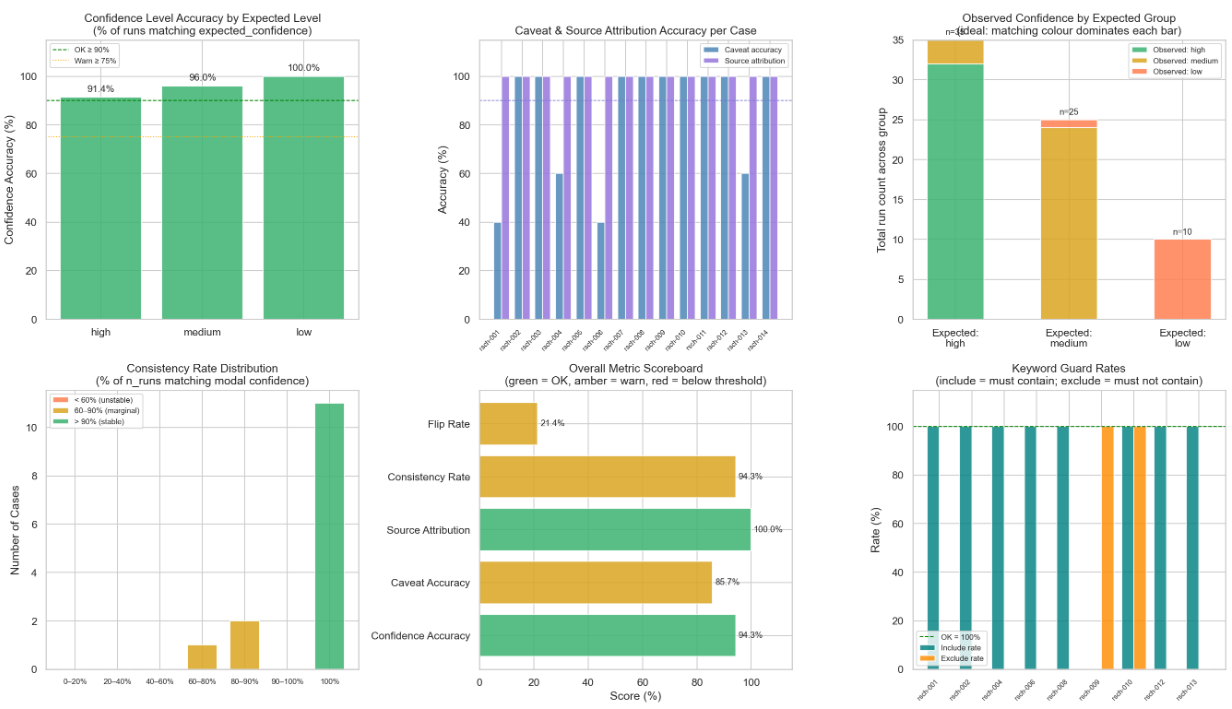
\includegraphics[width=0.8\textwidth]{fig4.png}
    \caption{Metrics for Search Results in Research Agent}
    \label{fig:research-metrics}
\end{figure}
\begin{figure}[H]
    \centering
    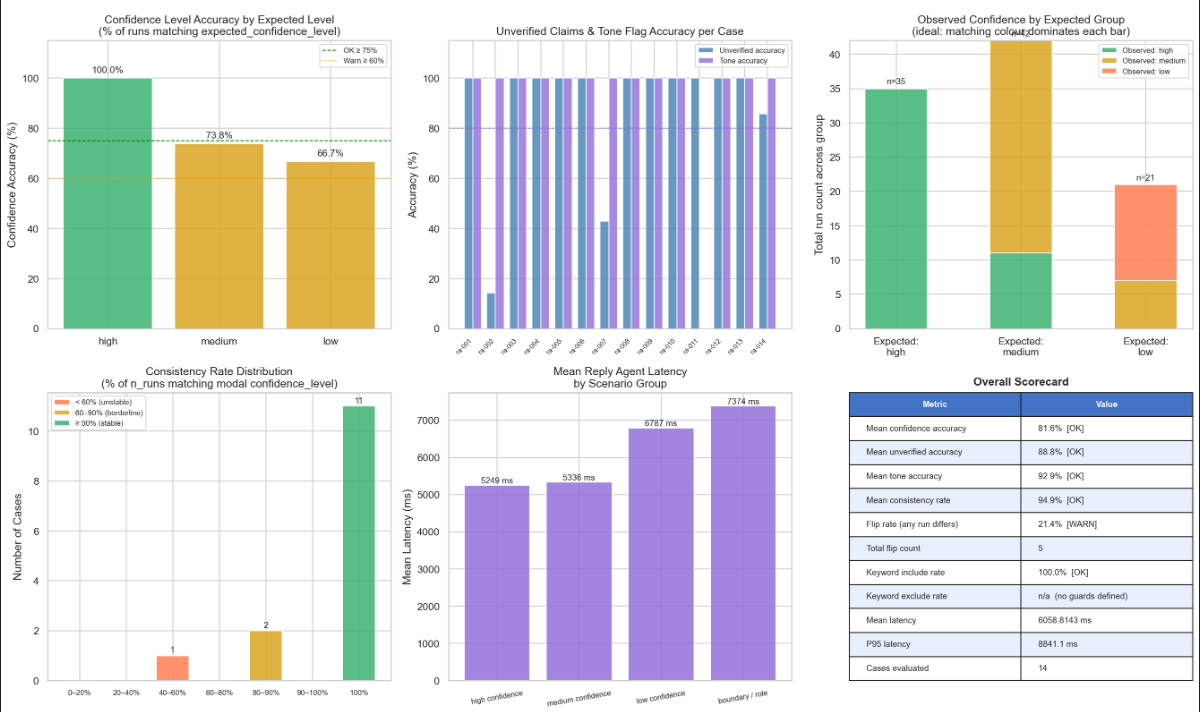
\includegraphics[width=0.8\textwidth]{fig6.png}
    \caption{Metrics for Reply Generation Results}
    \label{fig:reply-metrics}
\end{figure}
\begin{figure}[H]
    \centering
    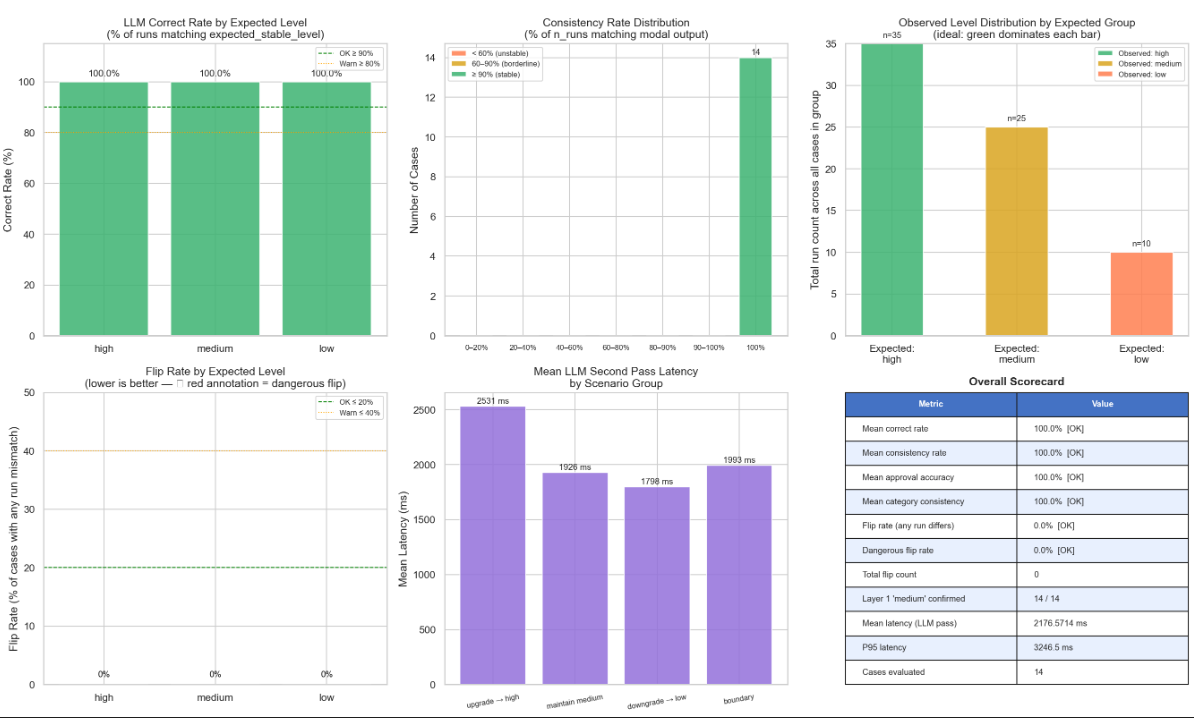
\includegraphics[width=0.8\textwidth]{fig5.png}
    \caption{Metrics for Risk Classification in Risk Node}
    \label{fig:risk-metrics}
\end{figure}

\subsection{Control-Flow Guarantee Coverage}
\label{app:eval-coverage}

\begin{table}[H]
\centering
\small
\renewcommand{\arraystretch}{1.18}
\begin{tabular}{|p{4.1cm}|p{3.0cm}|p{4.3cm}|}
\hline
\textbf{Guarantee} & \textbf{Evidence source} & \textbf{Current evidence} \\
\hline
Low-risk reply can be dispatched autonomously & Pipeline integration suite & Mocked end-to-end integration test passes for automatic low-risk dispatch. \\
\hline
Risky reply is held for owner approval & Pipeline integration + approval-rules suites & Approval routing and hold-for-review behavior are validated under explicit commitment and discount-trigger cases. \\
\hline
Parallel fan-out results are aggregated before reply synthesis & Pipeline integration suite & Mocked end-to-end integration test passes for orchestrator fan-out/fan-in aggregation. \\
\hline
Sub-agent failure is quarantined rather than silently ignored & Pipeline integration suite & Mocked end-to-end integration test passes for failure quarantine with pipeline completion. \\
\hline
Identity resolution defaults conservatively and preserves mappings & Identity-resolution suite & Existing and unknown senders are resolved with conservative customer defaulting and mapping persistence. \\
\hline
Risk rules escalate explicit confidentiality, PII, and commitment issues & Risk-node and P2-risk suites & Deterministic and semantic risk suites validate escalation, aggregation, and fallback behavior. \\
\hline
\end{tabular}
\caption{Control-flow guarantees that are currently validated by the committed deterministic and integration suites.}
\label{tab:control-flow-guarantees}
\end{table}

\begin{figure}[H]
    \centering
    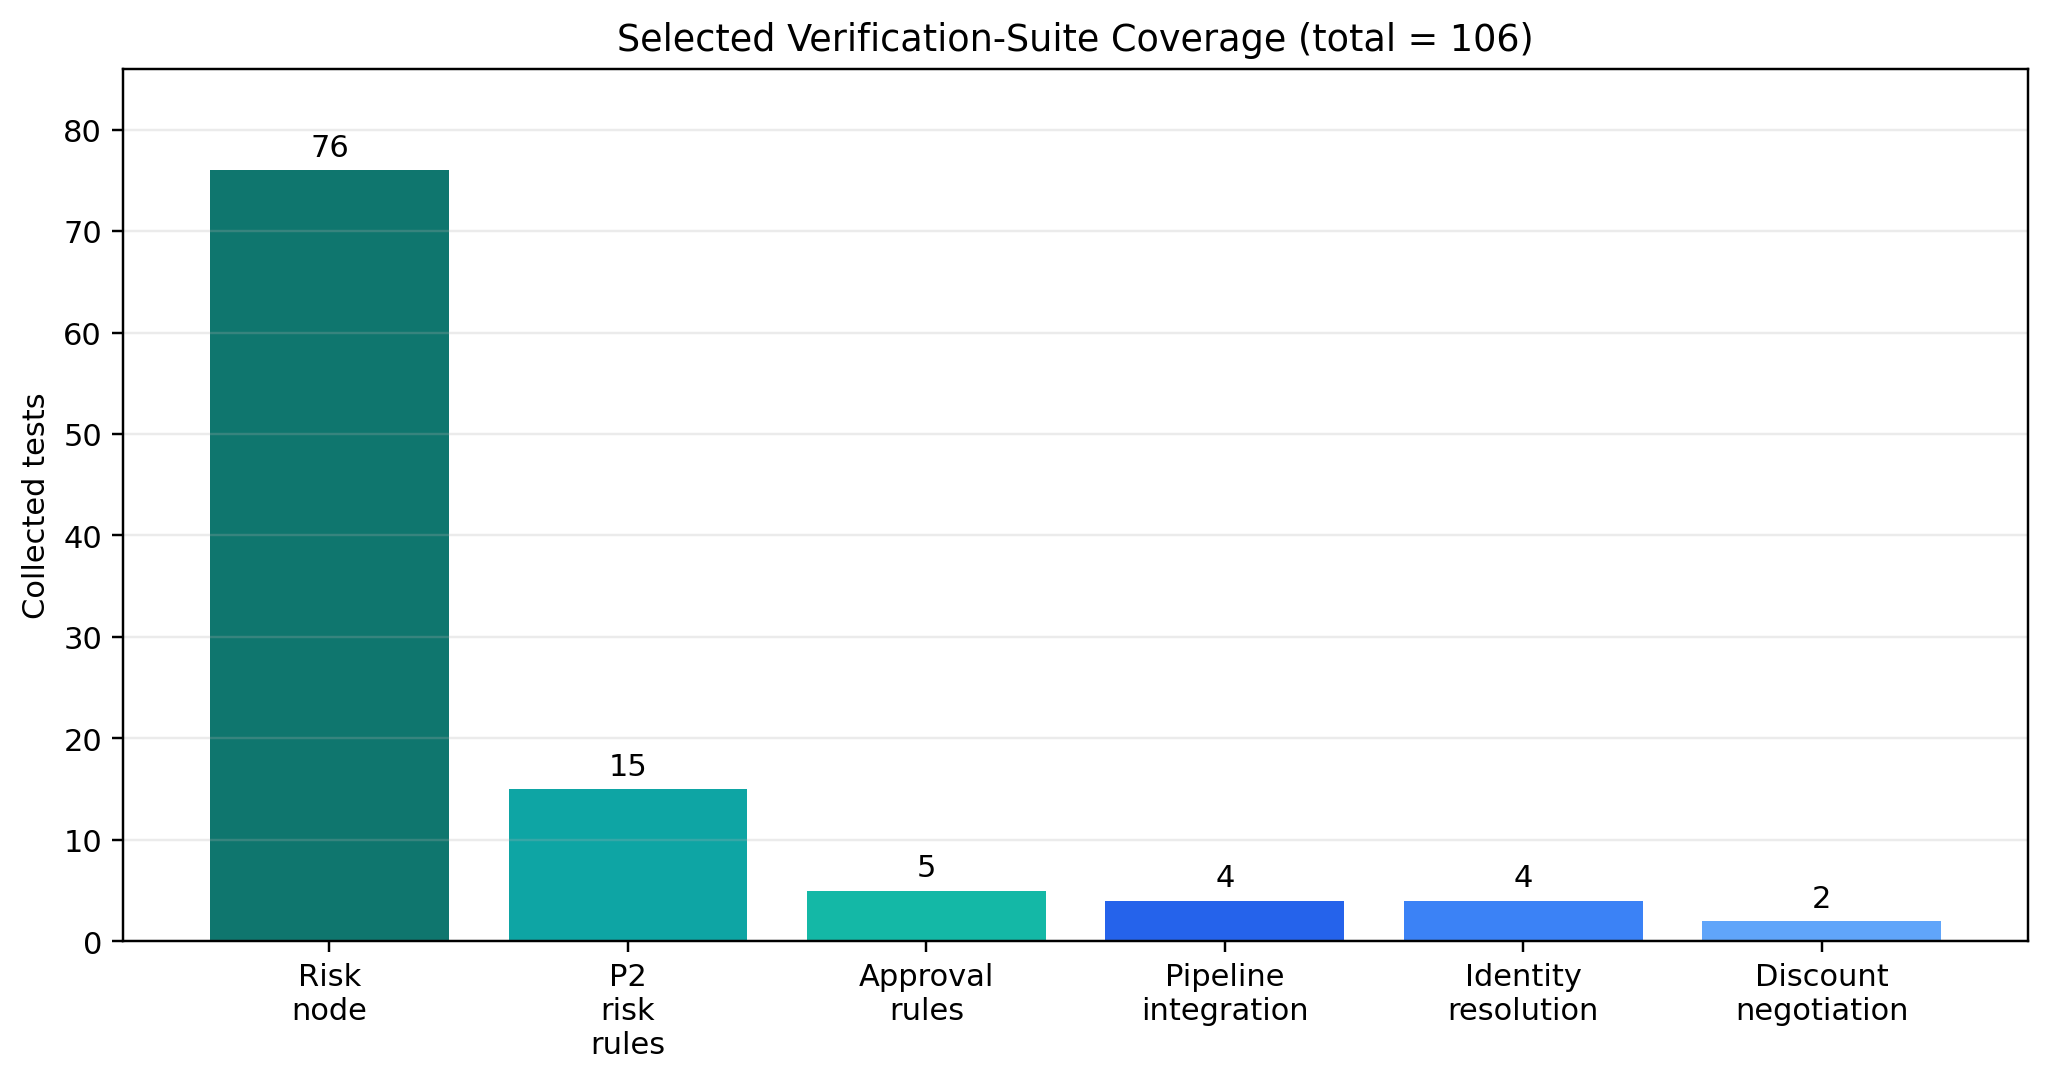
\includegraphics[width=0.92\textwidth]{appendix_test_coverage_summary.png}
    \caption{Verification-suite coverage summary generated from collected tests in the selected deterministic and integration suites. The figure shows the current distribution of 106 collected tests across control-critical modules.}
    \label{fig:appendix-test-coverage-summary}
\end{figure}

\subsection{Threats to Validity and Fair Baseline Design}
\label{app:eval-validity}

\paragraph{Baseline comparison scope.}
The paper includes a structured comparison against single-agent alternatives, while a fuller baseline study would compare against a strong single-agent assistant under matched tool access, the same policy corpus, the same conversation inputs, and the same evaluation protocol for verdict quality, latency, escalation behavior, and human-judged reply usefulness.

\paragraph{Human evaluation scope.}
The communication-facing nature of the system means that usefulness, trust, and stakeholder satisfaction are especially suitable for human assessment. Owner-authored SOUL strengthens this by making style and tone more explicit, transparent, and editable than hidden prompt-only control, and it can be complemented by future studies with real human raters or live users.

\paragraph{Scope and sample-size considerations.}
Some slices in the policy benchmark are small, especially supplier cases, so category-level conclusions are best interpreted as directional rather than exhaustive. In addition, the strongest end-to-end evidence currently comes from mocked integrations that isolate workflow guarantees clearly.

\paragraph{Methodological scope of the MEU framing.}
The approximate MEU interpretation is a conceptual lens for understanding the autonomy-versus-escalation policy. It is useful for explaining why bounded replanning, approval gating, and risk thresholds fit together, but it is not a formal theorem, a learned utility model, or an optimality proof.

\subsection{Technology stack breakdown}
\label{app:techstack}
\begin{tabular}{|l|l|}
\hline
Component & Technology \\
\hline
Backend Framework & Python 3.11+, FastAPI 0.110+, Uvicorn \\
Agent Orchestration & LangGraph 0.3+, LangChain 0.3+ \\
LLM Providers & OpenAI (gpt-4o-mini default), Google Gemini (gemini-2.0-flash) \\
Embeddings & OpenAI text-embedding-3-small (1536 dimensions) \\
Reranking & mixedbread-ai/mxbai-rerank-base-v1 (cross-encoder) \\
Database & Supabase PostgreSQL with pgvector extension \\
Frontend & Next.js 16, React 19, TypeScript, TailwindCSS 4 \\
External Search & Tavily API \\
Observability & Langfuse tracing with LangChain callback integration \\
Deployment & Docker + Docker Compose \\
\hline
\end{tabular}

\subsection{Database Schema}
\label{app:schema}
\begin{itemize}
\item \textbf{Core entities:} profiles, customers, suppliers, investors, partners, and external\_identities tables with UUID primary keys and owner\_id foreign keys for multi-tenancy.

\item \textbf{Products and orders:} products (with description\_embedding as pgvector(1536) and HNSW index), orders, supplier\_products, and partner\_agreements with embedding-enabled semantic search.
\item \textbf{Policy storage:} policy\_chunks with pgvector embeddings, source file tracking, category classification, and hard\_constraint annotation for grounded policy retrieval.
\item \textbf{Memory and messaging:} conversation\_threads, messages, conversation\_sender\_memories, memory\_entries, conversation\_memories, and memory\_update\_proposals supporting the three-layer memory architecture.
\item \textbf{Approvals and compliance:} held\_replies, pending\_approvals, reply\_review\_records, and owner\_memory\_rules providing a complete audit trail for all human-in-the-loop decisions.

\end{itemize}
A visual overview of the schema is provided in the \href{https://mermaid.ai/live/edit#pako:eNqtGdlu2zjwVwwVfVO7ko_4KHYB15GBYNsmSLoFdpNAkCXaJiKLKiXFdYv--w4pkqIuW26al4hDcjj35R-GTwJkzIx1SPb-1qNp7_PlQ_QQvX7d-7Ptj-8uSPSMaOKlmES9P3ofUZJ4GxxtTl1NstWGevG2t7j-9OW-DcvjQ9SDP1_bdtMtRV6Q3D8YTeD8ws3fsx4O8m-yjxB15So_5qaHGAkATkPxmaAogKPoW4po5IXqjoBH3q58kJLKTZBcFKEwh4Vekro7zglyvVRwAq-nKFDrLA7k2nhkAq-xu0M7QjGq8Svhpxhewk6DoNQ-ikACB40XAVDMZ7udRw_54gkd9oRKKW-9OEaRxo3GXQs3QlBtTFW2X8rbCxSqcy2V6JMsSt0ERz5yc8Ud0TQH5mjw92YZtVuAQMbkIz9_kyy6iyDAFPkMk1JjCqbRVdHCHXtv3vzVO2K33e40mkXr1UJicK1bEMuSlOwAGcSeaxrkHzeUBJmfJp0j2d38g3N3fxSXjGfyDLN_-X1KwYWq0M7DIsjEWxIhKY9d7EXCZJPUSzOBMqZojSgCqxWISCplyI2UadbzW8wzRSEC9nZuluhRVIcWhCkwBMKUHS6Mg3BRAL_5RydrFpIpAeNckgr2NfN4vBIEkBTcPKZY8spfcwtX1eVSitaNFi0eY2THyhq6ailAiU9xXHhQgsIQcppOnk9A_toaGPaf3CjbrRAtkeDCzSdxB-jcEBmbjoSTKhUuArRBwJKz5rTKXJnr6MqRHJc2unrUFfgmIKbdvefq0xfn7vO9uihcBcs16AAXSF_mKmviSyPQnKFkG03mIN93pVJ2KAXd6aRVt7rYedWkmVG0WgwlWCgWGDu4iReipIMFcyW2E9lVrTdQGUboDK3ezG8_f3Ju7-7lTaHWWCyZZymcL1OqwKOVdufoVt72NhShHSQ6jTQN2Emf4paE1QKBQqfRStEzijLkJlB8IzeW4RjopqkWv0BR2gonLgRu_Fznt9ntT7MvLYOikCdWXQq1vV8RRpPBM1ghE-UGR-jM7blNPY2HWqgvOcips7X3Tt3q6ld3WRyH-BzHuvvn5ubDFfMsdfdRlq5iDapLCrwvLC7KSQcqBgqW557jYZIWV8uqNVgXk1KXjtkUP3So59Y9cldZhQ1RC_G-EO8QONghqTDK_bAC48o97ob8s5MDKk1xk2qRS8lYG850NbePrJA-QF16FeTdHitRSYj9Q2f7--h8vL79974d06PsZNgBkFUq-r0y4JS-z-5aBPoisJb6llJbl3ob8T7exYSmnqqQGzUk-mKtda1ATvFyqtP-3aS3t5daQ8xpEOzUoSdZqnbWClBwcYpt8B7w0oI38TqTa-oB8d4RneTUCMHRLOR81IGn2Choq8e5pp63XbIxt33of7LoiedOfX3S2ElGfeSucahKmg0qdQMcj4vB5r_pgBTELq1ktYU4VsSaEj9QWwSs3UsggGHJV5folBebAYauOgWu9OXJgZs2X9NNmOLkqfHFrkFsHkPge_ZCiDi36BmjfW8Zkn3nADa_ubm9_jL_cHffjKgcv3Jls1AbE6i5tUBW3TkpD49uEFR-3kqKRUDkgRwT4ooqrA9klMj6kYnODaFgDI-mXllXAkc1MwUhs8bCE6xzU63CztEsD8Nq3MCe1JkpxYNzqBeZPUehp_stCgMotFiKL40ZFDwPafqy42T4lzNPTk3hilU--Xodqsit8y20RPWCqpsm81fzPfjns-ksMN4EPikAqGrQ7xOHt5cz0V-Tj7RDHsL1DYq-ZphCXSVPiKYes7wTIB8nqtMSAgi9lXpFSlp3qLpFKbAc6zZ0JUe00hIb8nah2c90Uz3rXLuq5SD0yLHOjT8lLC1BiFyQaI03GfXyfrbrHOD2enn1wblvwfOoogXbFfM2_lk32nUWhprhrbIER8BoE6jWeasdSKEZZMFDBczK_-_FRIEPTikoN_SiTaYsOUBrLwtTYS2pOi98QKQ5PpNOtiQMVC-A19jPW0NXa7MqGxHLDEG36Z6wM54pVAlAsrAM4Q5UgqhB7YpAKiJPKKrA92i1JeTJTRCQcF5eXoRekqCEqziEiuZkT-uzC5dozSf64MZhOHvlDJb95aUJKgLiZq9sZzJxRmL5Zo-DdDvrx99MH16gs1fW5XA8t99pqPhcTOKaLEfOVOEaDubWcNyKy34_cvqWjisfmwlky-Vy4tgK2XI6n_TbCVuOxkt7rCMTwwKJbeCMliOFbeL0h_N5K7bh3B5OFiU2RQ9YEDdwrIK495OFZbWicy5GtlXiNDcnKbaFs1wWnI6GF864nbb-xaA_mOjIZNxStDnvHUehc0aD6aBdcO_H9sIusSoCgiTOWo6Xc4XNsuaLhd1uH9aFdTF8x8yX42v87chs_JnKPPZDlKkiLDv1TmGXM3UzH5ubqm_nZqnOqXm22TaZFUfUDTnZMuujKLN1DCVvKSxq1mDWZghqTx0u9-tmpec1G5pGs96AmaU-yNT7B_FA9b1q6jRr6dDUM6HZlN6UCRbyE1lFfrwzTGNDcWDMUpohE2p6CnEZlsYPFhAfjHQL0n0wZvApov6D8RD9hGuxF_1HyE7epCTbbI3ZGgiDVU79JfZYMFVHuPEs2I_Ixqxv2RyHMfthfDNmk-nbqTWyh9O-NR3ao7FpHIzZm6n9tj8cjIe2ZU-ng8lo_NM0vvNHrbfTsX1h9e2BNbAHY3t08fN_3yF-VA}{Mermaid diagram}.

\subsection{Multi-Agent vs.\ Single-Agent: Detailed Comparison}
\label{app:comparison}

The table below provides a precise, dimension-by-dimension comparison explaining
why our multi-agent architecture yields superior correctness, safety, and auditability
compared to a single-agent LLM assistant.

\vspace{1em}
\noindent
\renewcommand{\arraystretch}{1.4}
\begin{tabular}{|p{2.2cm}|p{3.8cm}|p{3.8cm}|p{4.6cm}|}
\hline
\textbf{Dimension} & \textbf{Single-Agent LLM} & \textbf{Our Multi-Agent System} & \textbf{Why Multi-Agent Wins} \\
\hline
Separation of Concerns
  & Single prompt handles planning, retrieval, policy, risk, and memory simultaneously.
  & Dedicated agents: Retrieval, Policy, Research, Memory, Risk, Orchestrator.
  & Context is separated; this allows failure to be local and each agent is independently testable and replaceable. \\
\hline
Safety Enforcement
  & Access control embedded in system prompts, no absolute boundary restrictions.
  & RBAC enforced at tool-binding level, independent of LLM behaviour.
  & Hard security boundary cannot be bypassed by adversarial inputs or model drift. \\
\hline
Risk Governance
  & No structured risk layer; safety relies entirely on in-context instructions.
  & Two-layer pipeline: deterministic regex rules + LLM semantic analysis.
  & Catches both explicit violations and implied or nuanced risks. \\
\hline
Human Oversight
  & No structured HITL workflow; all outputs dispatched immediately.
  & Medium/High-risk replies held for owner dashboard approval before dispatch.
  & Owner retains control over binding commitments, concessions, and sensitive disclosures. \\
\hline
Auditability
  & Minimal; hard to trace why a specific response was generated.
  & Full audit trail and Langfuse tracing.
  & Every decision is logged, reviewable, and attributable to a specific pipeline stage. \\
\hline
Coherence
  & Limited; long-term memory lost across sessions.
  & Three-layer memory: short-term buffer, durable summaries, sender-specific profiles.
  & Coherent multi-turn context maintained across sessions without exceeding token budgets. \\
\hline
Policy Grounding
  & Policy knowledge baked into prompt; stale and unverifiable.
  & Hybrid RAG: pgvector semantic search + lexical search + cross-encoder reranking.
  & Responses are grounded in current, citable policy documents and can be independently audited against retrieved evidence with 90.9\% verdict accuracy on the current policy benchmark. \\
\hline
Extensibility
  & Adding new capability requires modifying a monolithic prompt.
  & New agents registered as LangGraph nodes.
  & Modular addition of Legal, Accounting agents etc.\ without touching existing agents. \\
\hline
\end{tabular}

\subsection{Additional Test Suites}

The following shows the detailed, comprehensive test suite covering unit tests and integration tests in the pipeline:

\begin{itemize}
\item Approval rule regex pattern matching (test\_approval\_rules.py)

\item Discount negotiation logic with quantity tiers and margin floors (test\_discount\_negotiation.py)

\item Identity resolution for various sender types (test\_identity\_resolution.py)

\item Intake node workflows (test\_intake\_node.py)

\item Rule-based risk evaluation (test\_p2\_risk\_rules.py)

\item Semantic risk evaluation (test\_p2\_semantic.py)

\item Policy RAG retrieval accuracy (\texttt{test\_policy\_tools.py}, \texttt{evaluate\_answers.py})

\item Retrieval Agent SQL retrieval accuracy (\texttt{test\_retrieval\_tools.py}, \texttt{evaluate\_end\_to\_end.py})

\item Full pipeline integration tests (\texttt{test\_pipeline\_integration.py}) covering low-risk auto-send, hold-for-approval, fan-out/fan-in aggregation, and failure quarantine

\item Error handling and safe agent calls (test\_safe\_agent.py)
\end{itemize}


\subsection{Team Contributions}
\label{app:contributions}

\renewcommand{\arraystretch}{1.3}
\begin{longtable}{|p{2.8cm}|p{10.8cm}|}
\hline
\textbf{Team Member} & \textbf{Contribution Areas} \\
\hline
Ewen & Served as the overall project orchestrator and technical lead. He defined the end-to-end multi-agent system architecture and workflow design, implemented the Orchestrator Agent and intake/receiver pipeline, integrated major backend control flows across the website and Telegram channels, contributed to memory and approval workflows, tenant isolation and authentication hardening, tracing and deployment integration, and coordinated cross-component integration, debugging, and final system consolidation. \\
\hline
Ng Chun Man & Developed the Message Reply Agent and Risk \& Confidentiality Agent, and defined the safety evaluation criteria used in the system. \\
\hline
Gabriella & Implemented the backend infrastructure, API and webhook integration, and frontend workflow and digest visualization components. \\
\hline
Jingyu & Designed the database schema, implemented data retrieval and logic for the Policy and Retrieval Agent, and contributed to the evaluation pipeline, including ground-truth generation, retrieval and policy test scripts, reranking and evaluation refinements, and unit and end-to-end performance benchmarking. \\
\hline
\end{longtable}

\section{Source Code Repository}
\label{app:repo}

The full implementation of the system, including backend services, frontend code, evaluation scripts, and test suites, is available on GitHub:

\href{https://github.com/EwenCheung/One-Man-Business-Multi-Agent-Orchestrator-System}
{One-Man-Business Multi-Agent Orchestrator System Repository}

\section{Demo Video}
\label{app:demo}

The demo video demonstrating the end-to-end system workflow can be accessed at:

\href{https://youtu.be/AAmxgg40FW0?si=SxDm1C5yMYnv5M_1}{One-Man-Business Multi-Agent Orchestrator System Demo Video}

\section{Presentation Slides}
\label{app:slides}

The presentation slides summarizing the system design, evaluation, and project scope are available at:

\href{https://docs.google.com/presentation/d/151UmyMhb4_M2kS_1uxL8sJY5ovF1HBeqFqsfzxMgCDA/edit?usp=sharing}{One-Man-Business Multi-Agent Orchestrator System Presentation Slides}

\section{Detailed Architecture Diagram}
\label{appendix:architecture}

The full-resolution architecture diagram, including the detailed control flow and component interactions, can be accessed at:

\href{https://mermaid.ai/live/edit#pako:eNqlWQtz2kgS_itTbO3V3kY2No6Nzd5tFbZlmwoGgiC57OVKNUgDaC0krR622ZD_ft3zkkbgOHZSlURoZnp6er7u_rr1peHFPmt0GouUJksyufwcEfjz88_k30_80RPsKE_XpEkuljSKWJh958qsmIm9nGvXHkzGn_77uSFEaUGN_4mp-OfKdqc9mHKVxlHOIp9Me_-apc3fB-wx3_8zIwldsAy08Gm2nMU09beWd0e4Xs0fx0XOyA2N_JClGRc1l6KbWeo1aZLA36D5qyFmcu1OHXvsoK6POUsjGpJppgRMWMjgTKv6ErGzGiXncU7glalf15mIaVc0y-GJnFPvDpThgmfieX9FgwjOCHrtB5HPHvkgV_P-sPkreUPUcy73qqgP6z9H33-r2s5N4hQJndGMveJir8bDwcQeXFYvrhRIup7Hsq2Lcqaj7nnXsauL9JKLMGBRLuw9S-MHMD5IhH_v-QP1V0FkCFTS3O50cgMiy82LfLnLOlX9L7uTLqwZpcGKAjIvaU5Jn65ZamwxGjqT67HtVKWP4ixfpMx53-eqJlICwAogmgt7GjC5GdvdSxThxRGcJaN5EEduvkwZrWH51rnGeSswHYLeHLNvuTf1bDFlFadrFwyWBjsmjsZDUL3br0wtEtCOuUkaJ3FGaz7owE3aYxeW1tXMwH4sdbmQ-k6jYb938cm9uJkO3uFOSRwG3tr1lkV0J-4xWdwzL49No573_nDt23MbsQPq-IWXo39nRZIABFK38i6haR7BKwoGZysNj4cgXxIhmbDVjPl-EC1quo2HV70-txXImwchE0ud4bQPgsfTvg3_CdsQD7H4mBuuTmbgzHkM3gnzHthsGcd3gEYvZbmxkf2fidvj18tk3HADHzQN8rq5buz-pXt5DjNvWOiTMUvCNfzrxRDS-NZLeO2mDK2QgcsnYHo4lwvISuN7uDJ4h6NrmHMfsAf4j681NhlOJ-fD6eDSBSxVoEQAmCHju0B4nMUFeN4yyMCA612ewmMy2dv7feNxryTUQzRkGxlu67P8AHTJCUc0misNcthzDtejo7ZF1L1aRJ_IItINNtXwoKWrF3wPCl7dzOA8oMjGdP7dC_iRyV8FQ-ButC9XzojRGGcGkYz4c5Z7S653_AC4I96S5oa6SZHCuwzlycAuhKn0wcUpo29kitBT1H4KTqjSdmSXo5Udvj-4y9wCNwHnznKyxDQIIHpFhB_b76e2M0FkK6ljKfVGSa0i76N9fjMcvqvmw4_ynDIZc_iBl6SAJlcd15XWAnD7zC8SfAhj786QDVZwewMQDfcHFlMGbgaRF0NaWMhIHGPScdVLJfmXf27JQsNj9IdQvpcECYPDMG0rLiyj94xoVyl1xHhIgjmJIDqgv3KfRDckwilNZ_w4gKjaHUEw-tDtw4ZDjiqFJ-VVRrKX_t8Uk9gmZX-CaxlTRNSqzdjpxgJAiDl1PdsDwrZqiZzGYTorAjhgT5rzVthgU1vwPajs02hxzXGljP0KPI56I7vfGyB5KOUNwR0BkSlPVmSkpBuZoFx3Ea8SyAR-RSG1RCBI_gAOdg-R_5f9_X0TO73BpPsOJfWinN4xMgBqzVfKkL8GFGRxWHBt3sjgRiBnUPlGXp1MSSrxmKAZXyCbKU8G0ai7APFCxZBGGM2zO54OkOtmIisYQsb2ZIzuwpAfINRKCWkcsr3MixOww-U5pLg43Err3DcwmVd3lrmcjLvXHPUpje7gAbiCH3h5bXuH754xCseoCJnQ-wCynnz_hvT7tyRbRzkcNdimMUicQM6tyNJjtKW2uBShQ4HJiNBTixUQs-BvVtNs1P_EdcPsWyrmp3SeC0PCWriXOV6phy4_D2mNXCiPdpFG4Em7yqPHBRCNUkmfQWIB54FMG3il34OKiwVQLFOznoPBcxxkd6WAFH_RBdCfhYJQnOADSOG2g9gDASmhNbJ9M-yj5ZYxMApIZ5pDlJI5KJmIYerYknFoRbcuZDoC3myXVzLlpLIUmsCh4KwQwB_2uOqSYAFq5H7yhaKhu6KWiC8yMaMfEh4DNtqTxTT1iwcx4ZhiQDzz1-hLSiw-c6FzGu2B32y4kzw1Bk7w9DLnqSEFWrUn7iBoFESeEMDgu9x1N1Iz6W7PTYEdn5uidv7WvJrWPHi4ecwp53ojXENtCI8yO1Shri6o-o5PQ_DKpfDExQMGCMdAE5KlhtSmgqPaghXzg2LVXAaLpVgIqEEeA9wyq6xHaKuzlLLEiVhepBHJckRaHiOSNjrfixW4ms_VZHsNfB2xH1KPob8w3DVLIC-z6uISm5y1SUYa73FCkFAoSOIIrQg0T1RTmvWJn3wFTpZ5FMwC583lrwlkAZMuGjsFoEyab_GRjUH3lY76iHLVN12cR3IkLpLGbFSZ8pL8XqM1c7j6VyT4Ck_S8RQqNaHdFcrcGYOdDxfVFQ5L7wNPhCMe_sTJm1I9pn8L2rQ1LAOUHhe_640fcadVruvwQlmmpsgv-S3foMJBd5ZZ8g7qt_NEXaTqCKlzU6hK7gNKZEOJ6JLGoyE4jclEZSAw3pneDkYtIV--q-4qIQWr8LxbwH9-2XeCeqcw0c3gnl7wakyj9lt7-yr9lLvXaEOTSMmKoYnxavX47Q3E6VSCN6OdivdCEje4bA7tGMFe0K7XZRvoiVHd-9kxXvZ5dgwa7Zwd47pvs2utbLfsGJINkh0jxp0ZI7vCWpnWN5xkA5REcwouTZILybebwD_gP3WF_3jiEnVydt73eWW3ohHSNMEs67NVmpa8U_S6iOh1bXbZzsjINbaqKwEigVffrZbYeEOljlVIjzU2tSXGzD7cOGVba57GK2WkTe0Gq2VgCCV8kciOyGxda4ZVV77g04LqsWciXKPnpQWYf_Wa0hAgZo8HPHNowU4peCwFG1XWyB50sSs_hJjbFV8csBwHVCGvfvNUX_Havu0NcN01Q14vOmqKkWO7CC16D7WD2fOcdD_0eN0hCiDRxWQziTVjar87uL6aOqrOnUN8M3fB_km9-TK2L3ui5PID0U_gJcyCkxLOwEQP757BT5Do70pHVUa9KUtkeS8babMai0RrYVEagUrmFE0i-RxeYG3NMZyEFzSyauPVzvbcik_gbNlM2pqqXVvfIlbjUOnuQaEEBQoP1LI0NlcqNy8XNlWpC4QNphd013aO6uvp6CFufKvdsinBAokZszUiFE-BQUDdvbQx34Ls7ZO5nIstcQkv2Chk_OhkHyKmwOVLXNBRDpTlayhapVfhs_5wRyA0hJ2f_Bmjc2ZleQpxo_PTof-W-afy595D4OfLTit5tLw4jNPOTwfzw3aL1sSpz0VSIjuYtyoSD1qnb732yySq9qTS0Zt7rF3qeHx6cOS_TKKGv9TRZ2cVHdveEWUvlKi5lZA4Z6zFWlqi77VOWicvk4ifrbS0-ZFXnnj29vjo4Oxl0lTcVBIP58fzMy3xbfv4-OR5iSWgKjh6FoBeCJ54yeZEfZv9Aaz9VhOpOPDrkVGXSLFPlP0AMOoC8UvhD9xjXZz69PQDF1kX6QHlCLxS5PPYPXpOpA590o7HrM1mWuTJrN06PdjWUr7AD0k0Tem6Q47J8dZGla1EWWWJOsmqfhVSWPvNmC2CsyUpjyXaT5aqvy2zTLKq1N8q-ZXEnCFZBRRLUFcLc6aFqcmCLAMPjqXSn8VzpWU2VizsjFhYzVuV1CegaO4jOZ9lfBSzZG1hYSVhVeoGy6gSrLImsAwWa2m-bymGZ0kub0nmblV5Ose0oZf6KGaJvoYl8pklUpUlEqSlUp7GsCFCmgyNw61hWF-3SBRWjaWcEmnMwVDDaizSwG908rRgVmPF0hXFn40vuOxzI18yJIkdePTZnBZh_rnxOfoKyxIa_RHHK7UyjYvFstGBpJzBL1EwXgYUq339NuWlyQUUtnmjcwQuzaU0Ol8aj43OXuuwdbh_cnZyenDcPmofHB5ZjXWj0zrYb5-dnhy0j1qHp-328Vn7q9X4m298tH9ycnj6FkbbxyfH7cOTo6__B2VjTUI}{View diagram}
\end{document}
